\documentclass[10pt, a4paper, italian]{article}
\usepackage[T1]{fontenc}
\usepackage[utf8]{inputenc}
\usepackage{amsmath, amssymb, amsthm, thmtools, amsfonts, mathtools}
\usepackage{nicefrac}
\usepackage{calc}
\usepackage[pdftex, hyperindex, plainpages=false]{hyperref}
\usepackage[nameinlink]{cleveref} %load before classicthesis (clash)
%\usepackage[nochapters,pdfspacing]{classicthesis}
\usepackage{siunitx}
\usepackage[siunitx]{circuitikz}

\usepackage[a4paper]{geometry}
\usepackage{float}
\usepackage{mdframed}
\usepackage{titling}
\usepackage{booktabs}
\usepackage{graphicx}
\usepackage{caption, subcaption}
\usepackage{xcolor}
\usepackage[italian]{babel}
\usepackage{pgfplots}
\usepackage{listings}
%\usepackage{lmodern}
\usepackage{url}
\usepackage{enumitem}
\usepackage{tikz} %loads after classicthesis (xcolor incompat)

% lets graphicx know path where figures to be included are found
\graphicspath{{../figs/}}
\makeatletter
\def\input@path{{../figs/}}
%or: \def\input@path{{/path/to/folder/}{/path/to/other/folder/}}
\makeatother

% tikz pgf plots setup
\usepgfplotslibrary{external}
\pgfplotsset{compat=1.15}
%\tikzexternalize

% spaces and significant digits/figures for measurements
\sisetup{free-standing-units, space-before-unit, number-unit-product = \;,
scientific-notation = false, round-mode = figures, round-precision = 1,}

% turns all (hyperlinked) references black [default is blue]
\hypersetup{
	linktoc=all,
	colorlinks=true,
	linkcolor=black
}

% code listings config
%\lstset{
%language=Python,
%basicstyle=\ttfamily,
%columns=fullflexible,
%keepspaces=true,
%}

% mdframed (for boxed text) configuration
\mdfsetup{linewidth=0.6pt}

% Default fixed font does not support bold face
\DeclareFixedFont{\ttb}{T1}{txtt}{bx}{n}{12} % for bold
\DeclareFixedFont{\ttm}{T1}{txtt}{m}{n}{12}  % for normal

% Custom colors
\usepackage{color}
\definecolor{deepblue}{rgb}{0,0,0.5}
\definecolor{deepred}{rgb}{0.6,0,0}
\definecolor{deepgreen}{rgb}{0,0.5,0}

% Commands 
\newcommand{\executeiffilenewer}[3]{%
	\ifnum\pdfstrcmp{\pdffilemoddate{#1}}%
		{\pdffilemoddate{#2}}>0%
	{\immediate\write18{#3}}\fi%
}
% input .svg --> .pdf_tex graphs
%\newcommand{\includesvg}[1]{%
%	\executeiffilenewer{#1.svg}{#1.pdf}%
%	{inkscape -z -D --file=#1.svg %
%	--export-pdf=#1.pdf --export-latex}%
%	\input{#1.pdf_tex}%
%}
% Thanks UniPi's Department of Physics E. Fermi
\newcommand{\thanksdf}{(\thanks{Dipartimento di Fisica E.~Fermi,%
Universit\`a di Pisa - Pisa, Italy.}\;)}

% hyperlink to email address
\newcommand{\mail}[1]{\href{mailto:#1}{\textsf{#1}}}

% \vec for bold vectors, instead of overarrows (now "\arrvec")
\let\arrvec=\vec
\renewcommand{\vec}[1]{\boldsymbol #1}
% replaces straight phi with slanted phi
\renewcommand{\phi}{\varphi}
% replaces straight eps with curved epsilon
\newcommand{\eps}{\varepsilon}
% abbreviation for (sub_/super^)scripts of \lim, \sum,... in inline math
\newcommand{\ds}{\displaystyle}

% blackboard/number set letters
\newcommand{\CC}{\mathbb C}
\newcommand{\HH}{\mathbb H}
\newcommand{\KK}{\mathbb K}
\newcommand{\NN}{\mathbb N}
\newcommand{\PP}{\mathbb P}
\newcommand{\QQ}{\mathbb Q}
\newcommand{\RR}{\mathbb R}
\newcommand{\ZZ}{\mathbb Z}

\newcommand{\Abs}[1]{{\left\Vert #1\right\Vert}}
\newcommand{\enclose}[1]{{\left( #1 \right)}}
\newcommand{\Enclose}[1]{{\left[ #1 \right]}}
\newcommand{\floor}[1]{\left\lfloor #1 \right\rfloor}
\newcommand{\ceil}[1]{\left\lceil #1 \right\rceil}
\newcommand{\To}{\rightrightarrows}

% Math operators
\DeclareMathOperator{\divergence}{div}
\renewcommand{\div}{\divergence}
\DeclareMathOperator{\Imaginarypart}{Im}
\renewcommand{\Im}{\Imaginarypart}
\DeclareMathOperator{\Realpart}{Re}
\renewcommand{\Re}{\Realpart}
%\DeclareMathOperator{\arg}{arg}
\DeclareMathOperator{\tg}{tg}
\DeclareMathOperator{\arctg}{arctg}
\DeclareMathOperator{\settsinh}{settsinh}
\DeclareMathOperator{\settcosh}{settcosh}
\DeclareMathOperator{\tr}{tr}
\DeclareMathOperator{\im}{im}
\DeclareMathOperator{\sgn}{sgn}
\DeclareMathOperator{\diag}{diag}

\DeclarePairedDelimiter{\norm}{\lVert}{\rVert}
\DeclarePairedDelimiter{\scalar}{\langle}{\rangle}

% Logarithm with arbitrary base.
% -> log_10
\newcommand{\llog}[1][10]{\log_{#1}}

% Absolute value.
% -> |x|
\newcommand{\abs}[1]{\left| #1 \right|}

% Powers.
% -> x^a
\newcommand{\power}[2][2]{\left( #2 \right)^{#1}}

% Square.
% -> x^2
\newcommand{\sq}[1]{\power[2]{#1}}

% Expansion of the binomial coefficient.
% -> n1!/(n2!(n1 - n2)!)
\newcommand{\binomexpr}[2]{\frac{#1!}{#2!(#1 - #2)!}}

% Expression evaluation at a given point with square brackets.
% -> [x]_{a}
\newcommand{\at}[2]{\left[ #1\right]_{\makebox[-1pt][l]{${\scriptstyle#2}$}}}

% Expression evaluation in an interval.
% -> [x] _{a}^{b}
\newcommand{\eval}[3]{\left.#1%
  \right|_{\makebox[-1pt][l]{${\scriptstyle#2}$}}^{\makebox[-1pt][l]{${\scriptstyle#3}$}}}

% Upright d in math mode (for differentials).
% -> d
\newcommand{\ud}{\mathrm{d}}

% Differential.
% -> dx
\newcommand{\diff}[1][x]{\,\ud{#1}}

% Base command for defining derivatives.
% -> df/dx or d^kf/dx^k
\newcommand{\basederivative}[4][]{%
  \displaystyle%
  \ifx\\#1\\\frac{#4#2}{#4#3}%
  \else%
  \frac{#4^#1#2}{#4#3^#1}%
  \fi%
}

% Total derivative.
% -> df/dx(x) or d^kf/dx^k(x)
\newcommand{\td}[4][]{%
  \basederivative[#1]{#2}{#3}{\ud}%
  \ifx\\#4\\%
  \else%
  \mkern-4mu\left(#4\right)%
  \fi%
}

% Partial derivative.
% -> df/dx(x) or d^kf/dx^k(x)
\newcommand{\pd}[4][]{%
  \basederivative[#1]{#2}{#3}{\partial}%
  \ifx\\#4\\%
  \else%
  \mkern-4mu\left(#4\right)%
  \fi%
}

\newcommand{\intinf}{\int_{-\infty}^{\infty}\!\!\!}

\newcommand{\cinterval}[2]{\left[\, #1,~#2 \,\right]}

\newcommand{\linterval}[2]{\left[\, #1,~#2 \,\right)}

\newcommand{\rinterval}[2]{\left(\, #1,~#2 \,\right]}

\newcommand{\ointerval}[2]{\left(\, #1,~#2 \,\right)}

\newcommand{\prob}[1]{\displaystyle P\left(#1\right)}

\newcommand{\pvalue}{\emph{$p$-value}}

\newcommand{\cond}{\,|\,}

\newcommand{\expect}[1]{\displaystyle E\left[#1\right]}

\newcommand{\mom}[2][]{\displaystyle {\cal M}_{#2}\ifx\\#1\\\else(#1)\fi}

\newcommand{\momalg}[1]{\displaystyle \lambda_{#1}}

\newcommand{\momcen}[1]{\displaystyle \mu_{#1}}

\newcommand{\skewness}{\displaystyle \gamma_1}

\newcommand{\kurtosis}{\displaystyle \gamma_2}

\newcommand{\charf}[1][x]{\phi_{#1}}

\newcommand{\momgenf}[1][x]{M_{#1}}

\newcommand{\fwhm}{{\scriptstyle \textsc{FWHM}}}

\newcommand{\hwhm}{{\scriptstyle \textsc{HWHM}}}

\newcommand{\median}{\mu_{\nicefrac{1}{2}}}

\newcommand{\var}[1]{\ensuremath{\text{Var}\left(#1\right)}}

\newcommand{\cov}[2]{\ensuremath{\text{Cov}\left(#1, #2\right)}}

\newcommand{\corr}[2]{\ensuremath{\text{Corr}\left(#1, #2\right)}}

\newcommand{\like}{\mathcal L}

\newcommand{\likelihood}[2][]{\like\ifx\\#2\\\else(#2\ifx\\#1\\\else;#1\fi)\fi}

\newcommand{\chisq}{\ensuremath{\chi^2}}

\newcommand{\chisquare}[2][]{\chisq\ifx\\#2\\\else(#2\ifx\\#1\\\else;#1\fi)\fi}

\newcommand{\loglikelihood}[2][]{\log\likelihood[#1]{#2}}

\newcommand{\pdf}[3][]{#2(#3\ifx\\#1\\\else;#1\fi)}

\newcommand{\binomialpdf}[2][]{\pdf[#1]{\mathcal B}{#2}}

\newcommand{\multinomialpdf}[2][]{\pdf[#1]{\mathcal M}{#2}}

\newcommand{\poissonpdf}[2][]{\pdf[#1]{\mathcal P}{#2}}

\newcommand{\uniformpdf}[2][]{\pdf[#1]{u}{#2}}

\newcommand{\exponentialpdf}[2][]{\pdf[#1]{\varepsilon}{#2}}

\newcommand{\gausspdf}[2][]{\pdf[#1]{N}{#2}}

\newcommand{\chisquarepdf}[2][]{\pdf[#1]{\wp}{#2}}

\newcommand{\cauchypdf}[2][]{\pdf[#1]{c}{#2}}

\newcommand{\erf}[1]{\ensuremath{\text{erf}\left(#1\right)}}

\newcommand{\dccases}[4][]{#2 \ifx\\#2\\\else=\fi %
  \begin{cases}
    \displaystyle #3 & \text{per variabili discrete}\\
    \displaystyle #4 & \text{per variabili continue}#1
  \end{cases}
}
% sub/super-scriptable for all symbol as math operator 
\newcommand\Scaleforall[1]{\vcenter{\hbox{\scalefont{#1}$\forall$}}}

\DeclareMathOperator*\forevery{%
  \vphantom\sum
  \mathchoice{\Scaleforall{2}}{\Scaleforall{1.4}}{\Scaleforall{1}}{\Scaleforall{0.75}}}
\geometry{left=2cm, right=2cm, top=2cm, bottom=2cm}

% indexes subsections with letters, sections with numbers (1.a, 1.b, ...)
\renewcommand{\thesubsection}{\thesection.\alph{subsection}}

% lets graphicx know path where figures to be included are found
\graphicspath{{../figs/}}

\author{Gruppo 1.AC \\ Matteo Rossi, Bernardo Tomelleri}
\title{Es05A: Applicazioni non-lineari di amplificatori operazionali}
\begin{document}
\date{\today}
\maketitle

\setcounter{section}{0}

\section*{Misura componenti dei circuiti}
\begin{table}[htbp]
\centering
\begin{tabular}{cccccc}
\toprule
Resistenze $[\si{k\ohm}]$ & $R$ & $\sigma R$ & Capacità $[\si{n\F}]$ & $C$ &
$\sigma C$ \\
\midrule
\midrule
$R_1$	  	& 992 	& 8		& $C_1$ & 212	& 9 \\
$R_2$	  	& 992	& 8		& & & \\
$R_4$	  	& 991	& 8		& & & \\
$R_5$	  	& 9.96	& 0.08	& & & \\
$R_6$	  	& 99.9	& 0.8	& & & \\
$R_7$	  	& 9.96	& 0.08		& & & \\
$R_8$	  	& 104.6	& 8		& & & \\
$R_9$	  	& 103.0	& 0.8		& & & \\
$R_{10}$  	& 99.9	& 8		& & & \\
$R_{11}$  	& 1.911	& 8		& & & \\
\bottomrule     
\end{tabular}
\caption{Valori di resistenza e capacità misurate per i componenti dei
circuiti studiati. \label{tab: rcmes_B}}

\begin{tabular}{cccccc}
\toprule
Resistenze $[\si{\ohm}]$ & $R$ & $\sigma R$ & Capacità $[\si{n\F}]$ & $C$ &
$\sigma C$ \\
\midrule
\midrule
$R_1^Q$	  & 99.8 	& 0.8 	 & $C_T$ & 1.00		 & 0.04 \\
$R_1^T$	  & 9.94	& 0.08 	 & $C_F$ & 1.00		 & 0.04 \\
$R_2^T$	  & 2.19	& 0.03	 & $C_1$ & 99		 & 4	\\
$R_2^A$	  & 9.87		& 0.08		 & $C_2$ & 1.00		 & 0.04 \\
$R_3$	  & 10.01		& 0.08		 & & & \\
$R_4$	  & 9.91		& 0.08		 & & & \\
\bottomrule     
\end{tabular}
\caption{Valori di resistenza e capacità misurate per i componenti dei
circuiti studiati. \label{tab: rcmes_M}}
\end{table}
Dove gli apici $Q$, $T$ e $A$ indicano i diversi valori delle resistenze che
condividono lo stesso nome rispettivamente nei circuiti:
amplificatore di carica, trigger di Schmitt e multivibratore astabile.

Riportiamo per completezza anche i valori delle tensioni di alimentazione
continue per l'op-amp misurate con il multimetro
\begin{align*}
V_{CC} &= 4.99 \pm 0.03 \si{\V} \\
V_{EE} &= -4.99 \pm 0.03 \si{\V}
\end{align*}

Non è stato facile misurare i valori di capacità dei condensatori nel
circuito con il multimetro, che a volte con i soli puntali collegati legge
un rumore di fondo intorno ai $7 \pm 1 \; \si{n\F}$, abbastanza alto da
saturare il fondo scala da $\SI{2}{n\F}$ con cui si vorrebbero misurare i
valori delle capacità $C_T$, $C_F$ e $C_2$.

Per tutto il resto della trattazione come ampiezze dei segnali si intendono
misurate non ``picco - picco'', a meno che non venga esplicitato altrimenti.

\subsection*{Nota sul metodo di fit}
Per determinare i parametri ottimali e le rispettive covarianze si \`e
implementato in \verb+Python+ un algoritmo di fit basato sui minimi quadrati
mediante la funzione \emph{curve\_fit} della libreria \texttt{SciPy}.

%=======================
\section{Circuito amplificatore di carica}
\subsection{Progettazione del circuito}
Si è costruito un amplificatore di carica a partire da un op-amp TL081CP come
quello in \cref{fig: Qampschm}

\begin{figure}[htbp]
    \centering
	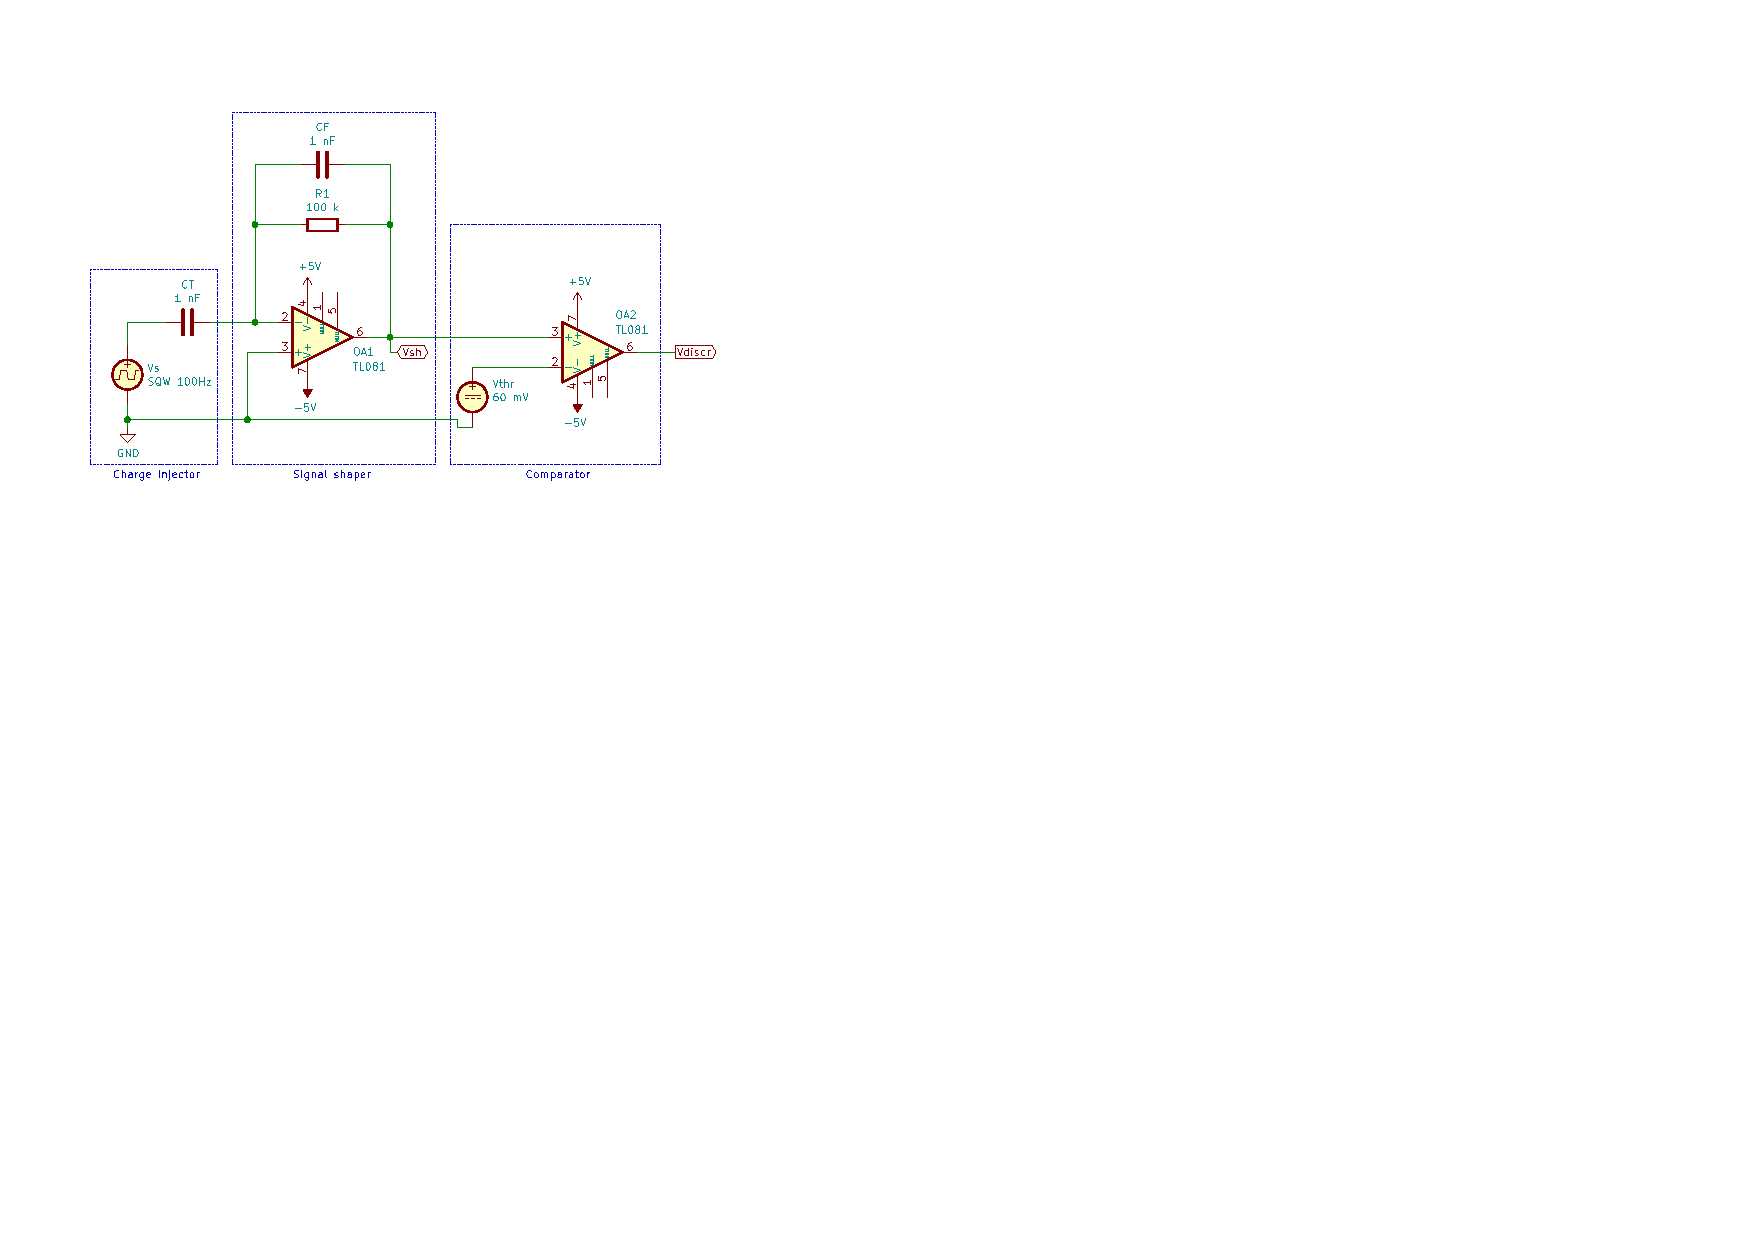
\includegraphics[scale=1.2]{Qamp}
    \caption{Schema circuitale dell'amplificatore di carica costruito.
    \label{fig: Qampschm}}
\end{figure}

In cui abbiamo indicato i sotto-circuiti di cui è composto, da sinistra verso
destra come: ``iniettore/rivelatore di carica'', ``circuito formatore/shaper''
(passa-basso/integratore attivo) e ``discriminatore/comparatore''.

\subsection{Funzionamento di iniettore e shaper}
Si è inviato all'ingresso di entrambi i circuiti un'onda quadra di
ampiezza $V_s = 999 \pm 8 \si{m\V}$ e frequenza fissata a
$f = 100.0 \pm 1.6 \; \si{\Hz}$, che corrisponde ad una carica
$Q\ped{in} = C_T \cdot 2V_s = 1.98 \pm 0.08 \; \si{n\coulomb}$, proporzionale
al ``salto'' di tensione dal livello alto a basso (e viceversa) dell'onda,
più semplicemente alla sua ampiezza picco-picco
$V_s^{pp} = 2 V_s \implies Q\ped{in} = C_T \cdot V_s^{pp}$.

Dunque abbiamo trovato come segnale in uscita dal circuito formatore un
segnale che dopo un breve transiente diventa un esponenziale decrescente,
con ampiezza iniziale $V\ped{sh} (t=0) = 2007 \pm 18 \; \si{m\V}$ e
con la stessa frequenza $99.9 \pm 1.6 \; \si{\Hz}$ dell'onda quadra.
Riportiamo in figura l'immagine acquisita dall'oscilloscopio con dettaglio
sul transiente al fronte di discesa dell'onda quadra.
\begin{figure}[htbp]
    \centering
	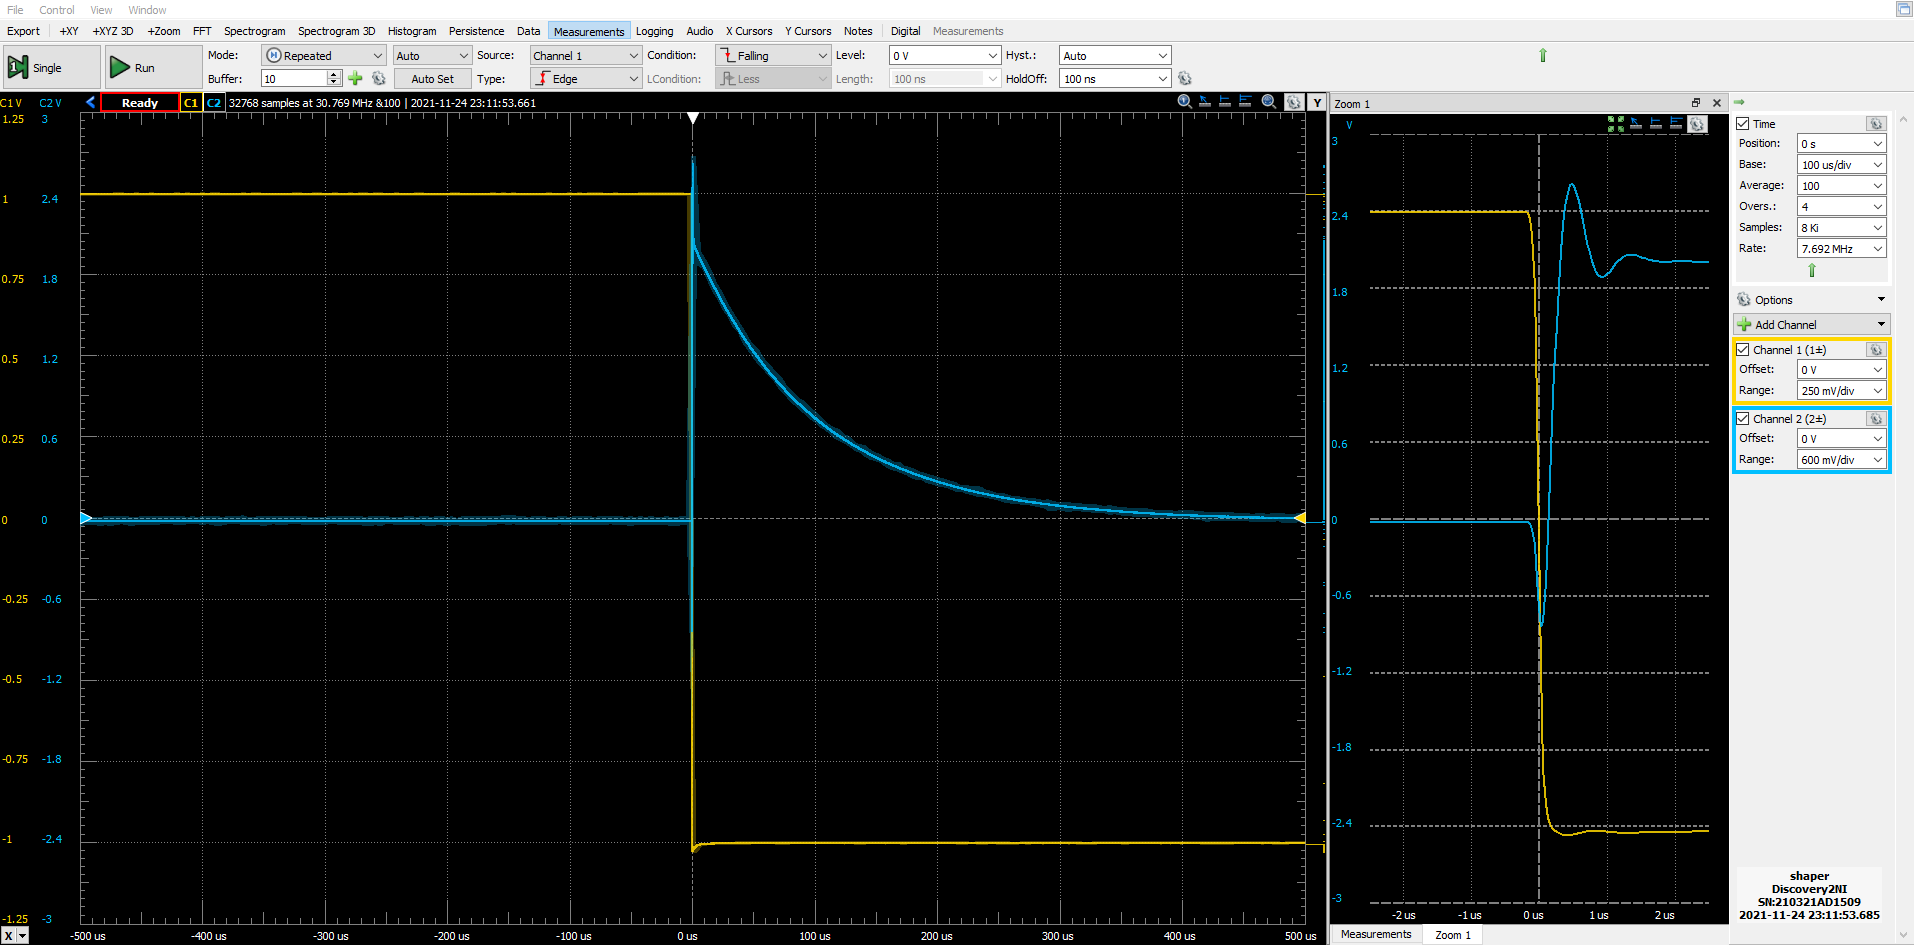
\includegraphics[scale=0.335]{shaperzoom}
    \caption{Acquisizione del segnale in uscita dal circuito formatore con
    un'onda quadra in ingresso $V_s = \SI{1}{V}$, $f = \SI{100}{\Hz}$
    \label{fig: shzoom}}
\end{figure}

Assumendo iniezione di carica istantanea sulle armature dei condensatori $C_T$
e $C_F$, il segnale in uscita dal sotto-circuito formato da $C_T$ e dal
formatore è legato al segnale in ingresso dalla relazione\footnote{Per una
derivazione più rigorosa di questo risultato si confronti l'appendice
in calce al documento.}
\begin{align}\label{eq: Vsh}
V\ped{sh}(t) &= \frac{Q\ped{in}}{C_F} e^{-t/\tau} =
2V_s(t) \frac{C_T}{C_F} e^{-t/\tau} \\
\tau &= R_1 C_F
\end{align}
Per i circuiti in esame i valori delle capacità sono
$C_T \approx C_F = \SI{1}{n\F}$ e $R_1 = \SI{100}{\kilo\ohm}$,
per cui possiamo semplificare il rapporto $C_T/C_F \approx 1$, da cui
ricaviamo come valori attesi
\begin{align*}
V\ped{sh}(t) &= 2V_s(t) e^{-t/\tau} \\
\tau &= R_1 C_F = 100 \pm 4 \; \si{\micro\s}
\end{align*}
Quindi complessivamente come tensione in uscita $V\ped{sh} (t)$ ci aspettiamo
di osservare una serie di picchi seguiti da decrescite esponenziali di segno
alternante con l'onda quadra in ingresso e di ampiezza doppia.

Questo risulta compatibile con quanto si è osservato dall'oscilloscopio, che
riportiamo per chiarezza in \cref{fig: shaper}
\begin{figure}[htbp]
    \centering
	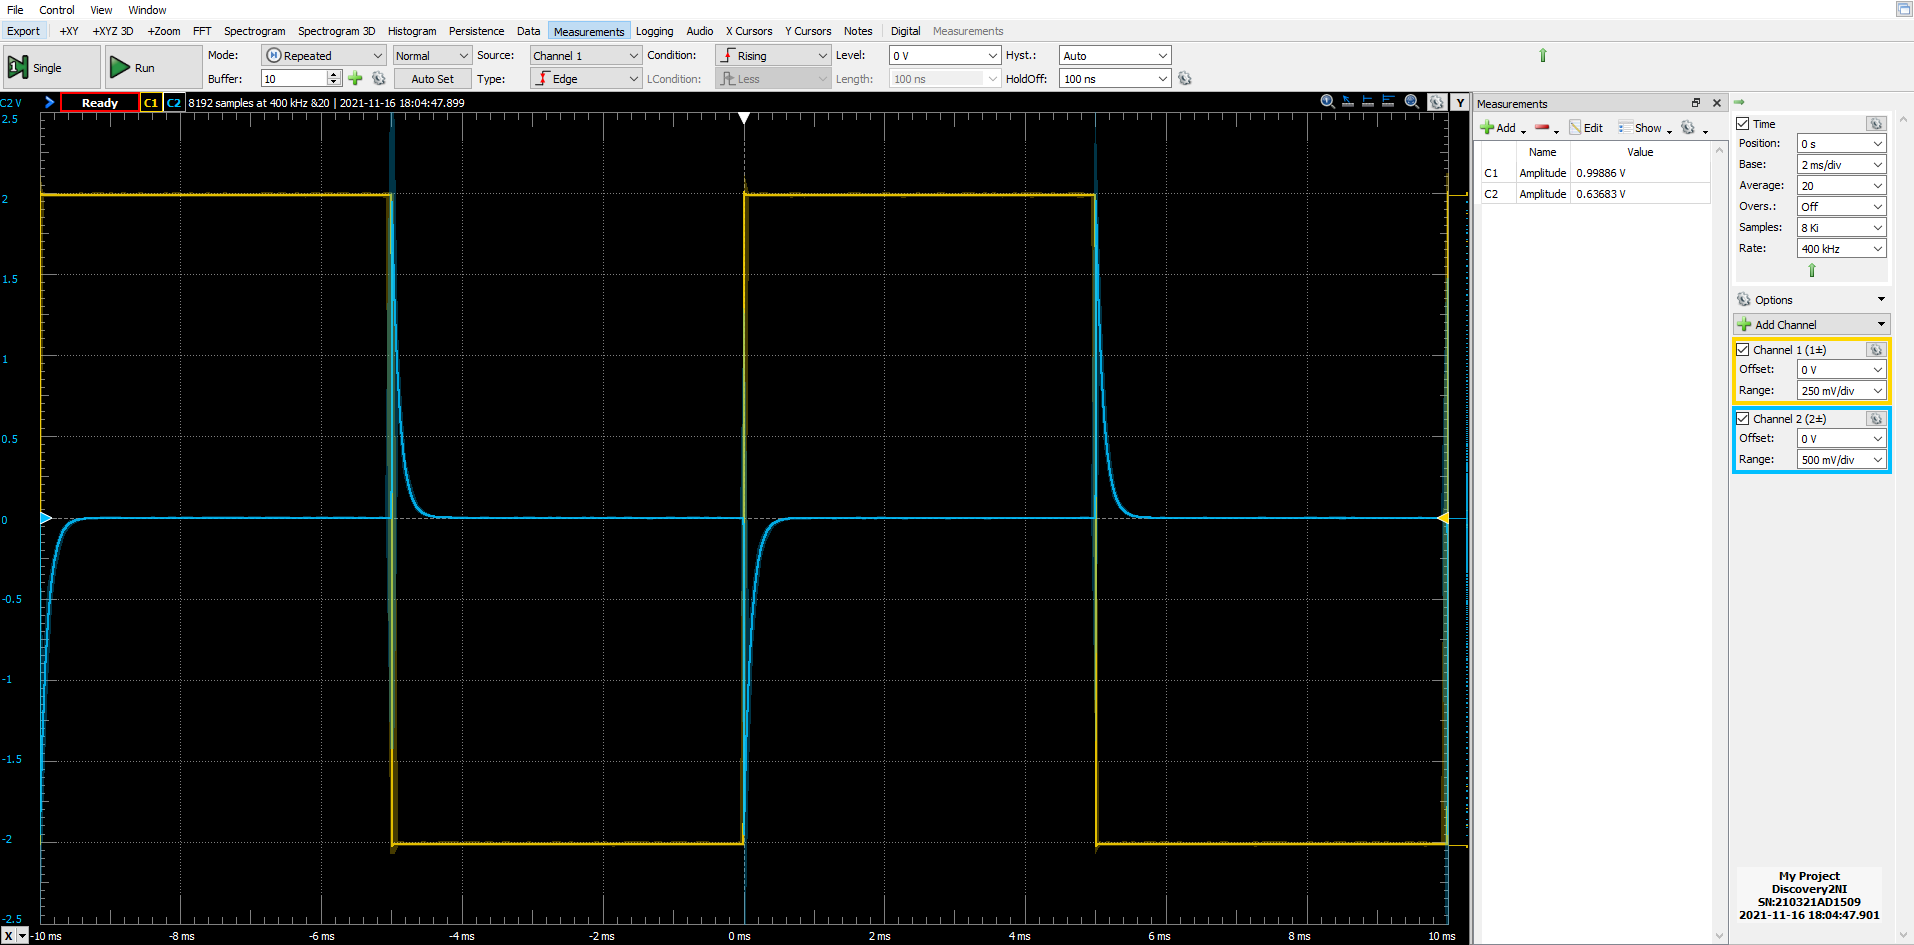
\includegraphics[scale=0.335]{shaper}
    \caption{Onda quadra in ingresso $V_s = \SI{1}{V}$, $f = \SI{100}{\Hz}$
    su CH1 e segnale in uscita dal circuito formatore $V\ped{sh}$ su CH2.
    \label{fig: shaper}}
\end{figure}

Dunque possiamo controllare che la forma d'onda esponenziale sia compatibile
con quanto atteso dalla \eqref{eq: Vsh} tramite un fit ai punti campionati
dall'AD2, di cui riportiamo brevemente i risultati
\begin{figure}[htbp]
    \centering
	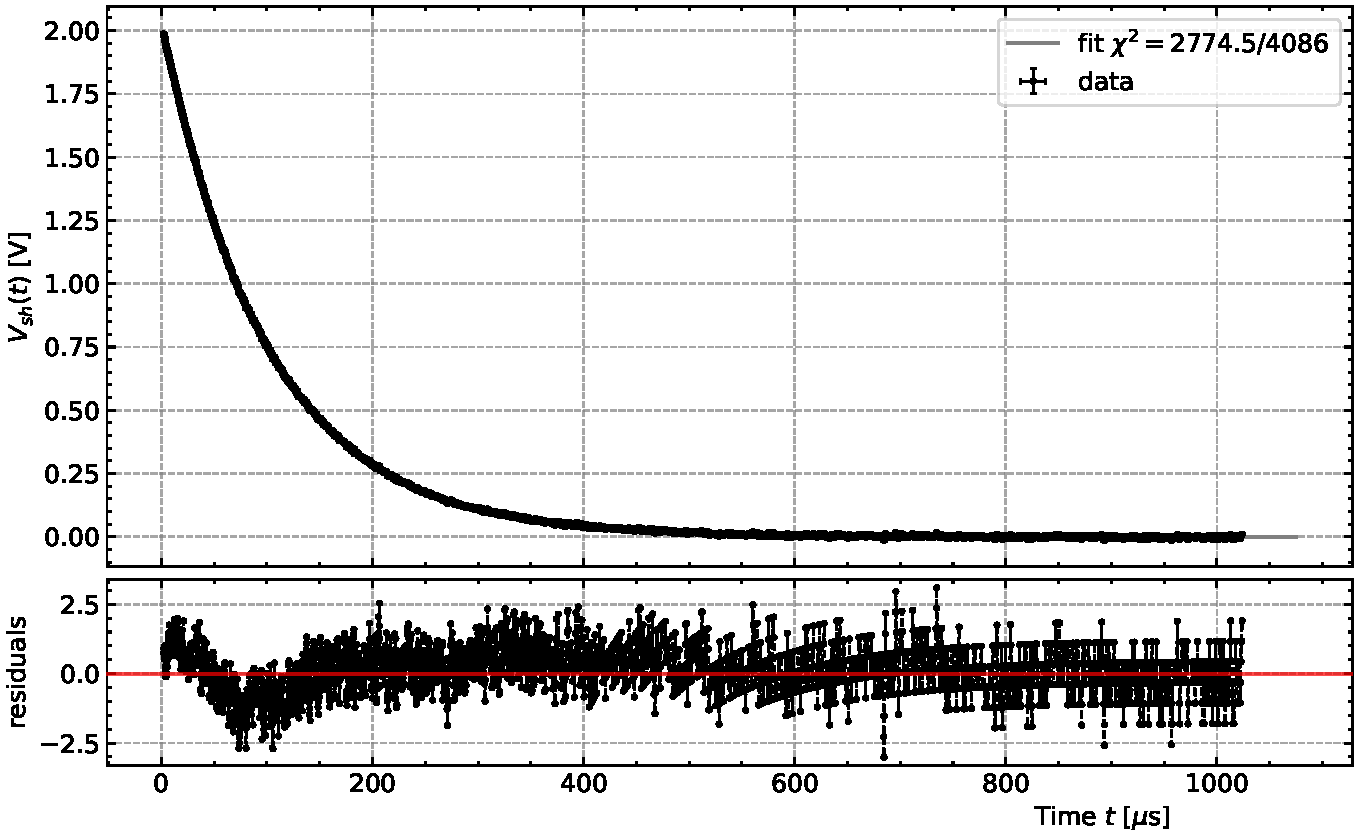
\includegraphics[scale=0.6]{tau}
    \caption{Fit con esponenziale decrescente al segnale in uscita dal
    circuito formatore $V\ped{sh}$ \label{fig: tau}}
\end{figure}
\begin{align*}
V\ped{sh} (t=0) &= 2021 \pm 2 \; \si{m\V}
&\tau = 101.88 \pm 0.03 \; \si{\micro\s} \\
\chi^2/\mathrm{ndof} &= 2774/4086 &\mathrm{cov_{norm}} = -0.75
\end{align*}

Da cui vediamo come non solo la misura di ampiezza iniziale sia compatibile
con il valore misurato, ma anche il tempo caratteristico di smorzamento $\tau$
risulta pienamente in accordo con il valore atteso dai componenti del
circuito.

\setcounter{subsection}{3}
\subsection{Funzionamento del discriminatore}\label{sub: discr}
Il sotto-circuito discriminatore è un comparatore con tensione di soglia
misurata con l'oscilloscopio $V\ped{thr} = 51.9 \pm 0.4 \si{m\V}$ e fornita
dal generatore di tensione (con valore nominale $\SI{60}{m\V}$) \verb+W2+
collegato all'ingresso invertente del secondo OpAmp.

Supponiamo di essere sempre in regime di saturazione per l'OpAmp ideale e
come prima assumiamo iniezione istantanea di carica sui condensatori. 
Grazie al fatto che le tensioni di alimentazione sono pari in modulo
$V_{CC} = - V_{EE}$ possiamo prendere come segnale atteso in uscita
\begin{equation}\label{eq: Vdiscr}
V\ped{discr} (t) = V_{CC} \sgn\left[V\ped{sh}(t) - V\ped{thr}\right].
\end{equation}

Più esplicitamente, ricordando che $V\ped{sh}$ ha ampiezza (iniziale) doppia
rispetto all'ampiezza in ingresso $V_s$ (o proporzionale a $V_s^{pp}$)
\begin{itemize}
\item se $V_s^{pp} < V\ped{thr} \implies V\ped{discr} = V_{EE}$ costante.
\item se $V_s^{pp} \geq V\ped{thr}$, ci aspettiamo (in un periodo dell'onda
quadra di durata $T = 9.99 \pm 0.16 \; \si{m\s}$)
\[
V\ped{discr}(t) =
\begin{cases}
V_{CC} & 0 < t < ToT \\
V_{EE} & ToT < t < T
\end{cases}
\]
In cui $ToT$ è il tempo in cui il picco esponenzialmente decrescente è
maggiore della tensione di soglia
$V\ped{sh}(t) = \frac{Q\ped{in}}{C_F} e^{-t/\tau} \geq V\ped{thr}$, appunto il
``Time-over-Threshold''.
\begin{equation} \label{eq:ToT}
ToT = \tau \log\left(\frac{Q\ped{in}}{C_F V\ped{thr}}\right) =
\tau \log\left(\frac{C_T V_s^{pp}}{C_F V\ped{thr}}\right) = 
\tau \log\left(\frac{C_T}{C_F} \frac{2 V_s}{V\ped{thr}}\right).
\end{equation}
\end{itemize}

Mantenendo lo stesso segnale in ingresso al circuito del punto precedente
(con ampiezza ben oltre la soglia $V_s \gg V\ped{thr}$) riportiamo il
segnale visualizzato all'oscilloscopio in uscita dal discriminatore in
\cref{fig: discr}.
\begin{figure}[htbp]
	\centering
	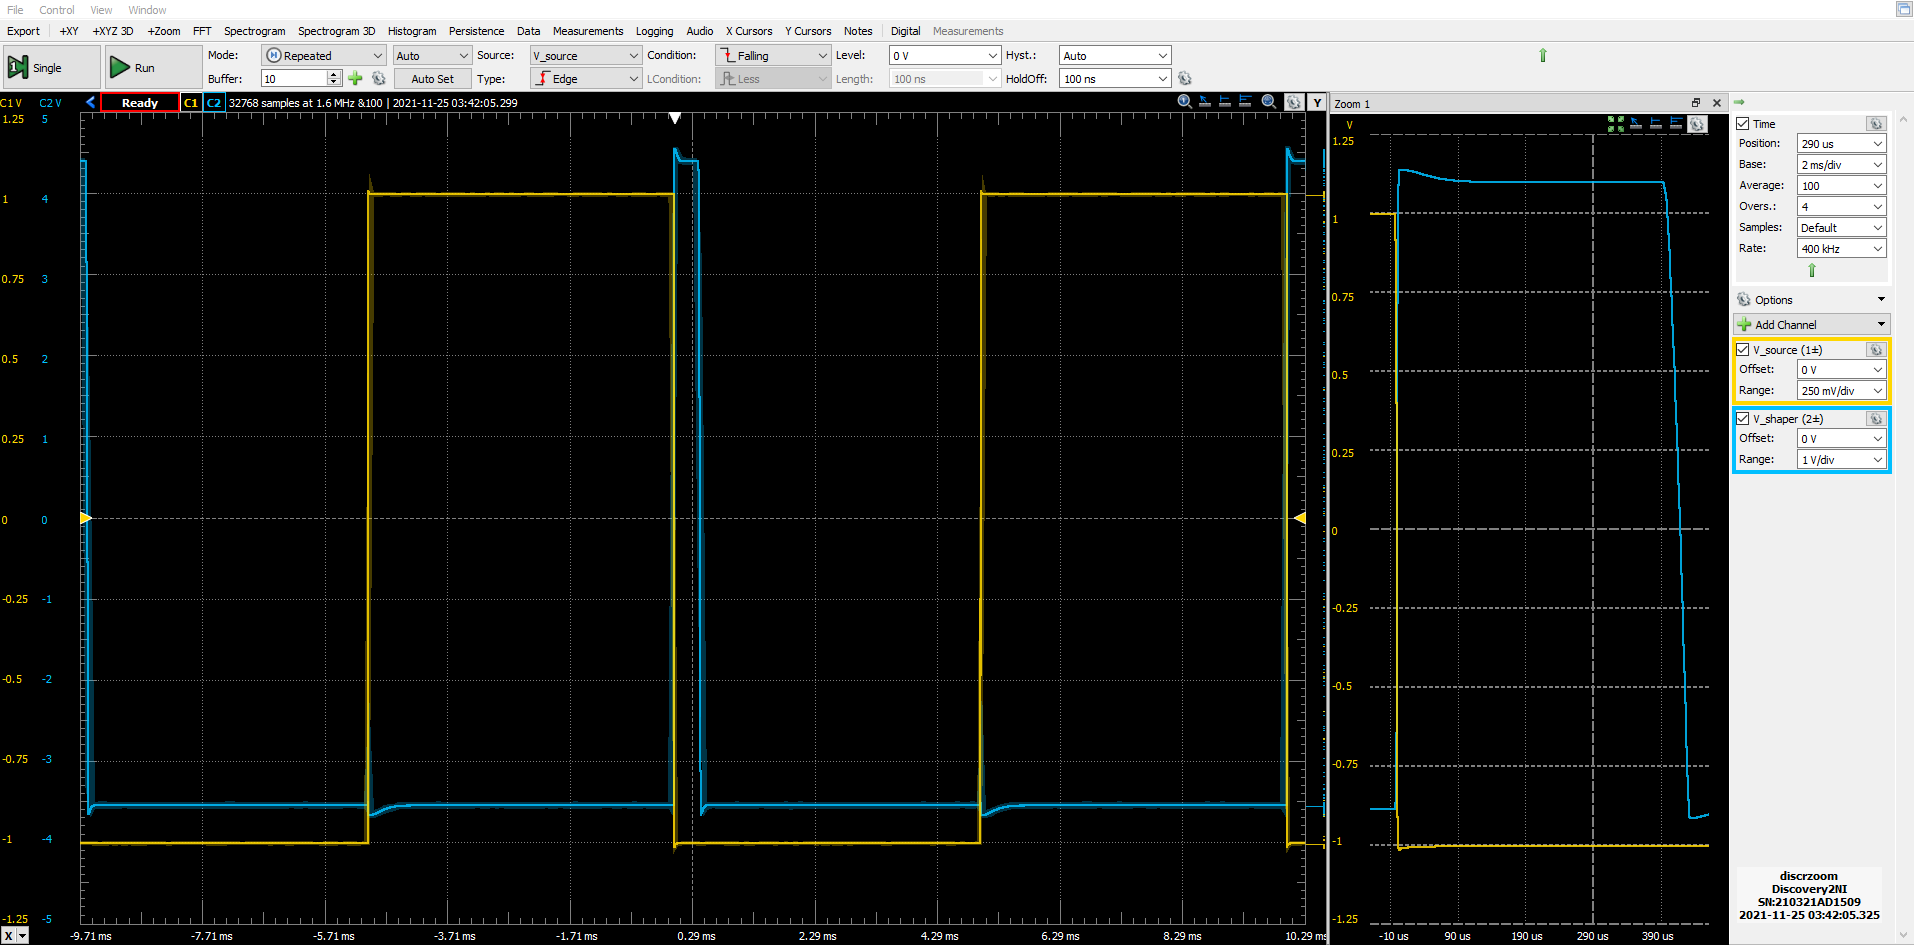
\includegraphics[scale=0.335]{discrzoom}
	\caption{Acquisizione del segnale in uscita dal circuito comparatore con
	un'onda quadra in ingresso $V_s = \SI{1}{V}$, $f = \SI{100}{\Hz}$
	\label{fig: discr}}
\end{figure}

Risulta già chiaro dal dettaglio a destra, in corrispondenza del fronte di
discesa dell'onda quadra, come il segnale in uscita non abbia né livelli basso
e alto simmetrici rispetto a $\SI{0}{V}$, né pendenza uguale (idealmente
infinita) nel passaggio tra questi due, al contrario di quanto atteso dal
nostro modello semplificato.

Possiamo caratterizzare il segnale $V\ped{discr} (t)$ trovato come un impulso
di tensione con livello basso $V_{OL}$ e livello alto $V_{OH}$ di durata
$T_{OH}$ che si ripete periodicamente con la stessa frequenza dell'onda quadra
in ingresso $V_s (t)$.
Riportiamo le misure dirette effettuate con i cursori
delle tensioni di saturazione del comparatore e una misura del tempo ``alto''
dell'impulso definita in maniera compatibile con la funzione automatica di
misura ``PosWidth'' (cioè come il tempo in cui la tensione si trova al di
sopra della metà del valore positivo dell'impulso, che quindi tenderà a dare
una sovrastima per la pendenza visibilmente non ideale dei fronti d'onda).
\begin{align*}
V_{OH} &= 4.38 \pm 0.03 \; \si{\V} \\
V_{OL} &= -3.53 \pm 0.02 \; \si{\V} \\
T_{OH} &= 382 \pm 5 \; \si{\micro\s}
\end{align*}

Osserviamo quindi che i valori di saturazione alta e bassa misurati non sono
compatibili con quelli attesi, ma sono entrambi inferiori (in modulo). Questo
può essere dovuto al fatto che in realtà il TL081 in regime di saturazione
produce al massimo tensioni entro il suo (Maximum Output) \emph{Voltage swing}
riportato come valore tipico nel datasheet $V\ped{OM, typ} = 13.5$,
sensibilmente inferiore rispetto al valore di tensione di alimentazione tipico
a cui è riferito $V\ped{CC, typ} = 15 \; \si{\V}$.

Quindi, volendo ragionare per analogia ci aspettiamo un'escursione massima tra
le tensioni di saturazione (date le nostre tensioni di alimentazione a
$\pm \SI{5}{\V}$) $V_{OM} = 13.5 \cdot V_{CC} / V\ped{CC, typ} =
13.5 /3 = 4.5 \; \si{\V}$, che risulta sicuramente più vicino a quanto
abbiamo misurato.

\subsection{Durata impulso per carica di test}
Abbiamo scelto come ampiezza per l'onda quadra $V_s = 999 \pm 8 \si{m\V}$ e
frequenza $f = 100.0 \pm 1.6 \; \si{k\Hz}$, dunque come carica
iniettata $Q\ped{in} = C_T \cdot 2 V_s = 1.98 \pm 0.08 \; \si{n\coulomb}$.
Si è scelta una frequenza abbastanza bassa, con periodo corrispondente a
$1/f = T \gg \tau$ di modo che tra una iniezione di carica e l'altra (cioè tra
ogni semiperiodo dell'onda quadra $V_s (t)$) i condensatori abbiano tempo di
scaricarsi, così da poter considerare indipendente ogni iniezione di carica
dalla precedente.

L'impulso in uscita ha durata pari a $382 \pm 5 \; \si{\micro\s}$ in un
circuito e $378 \pm 5 \; \si{\micro\s}$ nel secondo.

Per quanto riguarda il valore atteso per la durata dell'impulso, possiamo
confrontare i due valori trovati per il tempo ``alto'' con il valore atteso
di Time-over-Threshold
\[
ToT = \tau \log\left(\frac{C_T}{C_F} \frac{2 V_s}{V\ped{thr}}\right) =
370 \pm 15 \; \si{\micro\s}
\]

Che risulta compatibile con quanto abbiamo trovato sperimentalmente entro
l'incertezza associata.

\subsection{Andamento di TOT al variare di $Q\ped{in}$}
Provando con varie ampiezze del segnale in ingresso $V_s$, il comportamento
osservato per i due circuiti è essenzialmente lo stesso: per ampiezze maggiori
dei $\SI{50}{m\V}$ non sono presenti particolari deformazioni nel segnale
in uscita rispetto all'impulso atteso in uscita dal comparatore.
\begin{figure}[htbp]
	\centering
	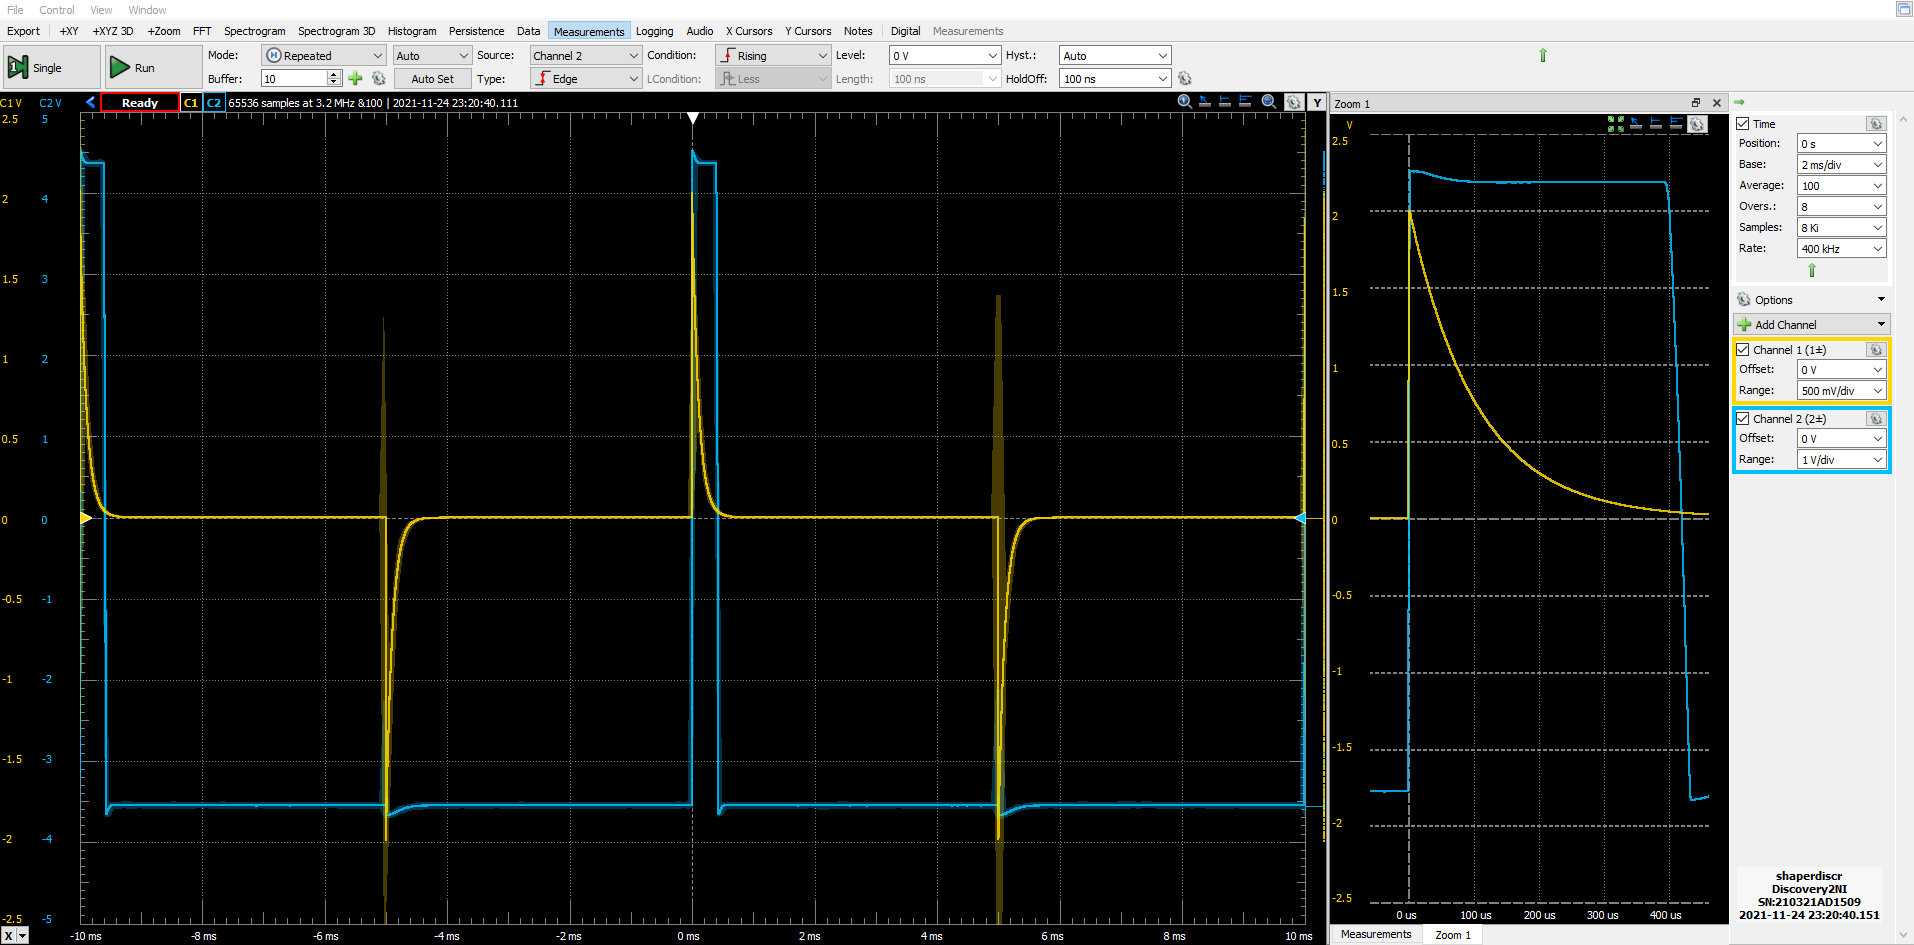
\includegraphics[scale=0.335]{shaper_discrzoom}
	\caption{Acquisizione del segnale in uscita dal circuito discriminatore con
	un'onda quadra in ingresso $V_s = \SI{1}{\V}$, $f = \SI{100}{\Hz}$
	\label{fig: shaperdiscr}}
\end{figure}

Riducendo l'ampiezza al di sotto dei $\SI{50}{m\V}$ il segnale in uscita
inizia a deformarsi, assumendo la forma di una parabola con concavità rivolta
verso il basso, la cui massima tensione raggiunta diminuisce in maniera
proporzionale all'ampiezza in ingresso.
\begin{figure}[htbp]
	\centering
	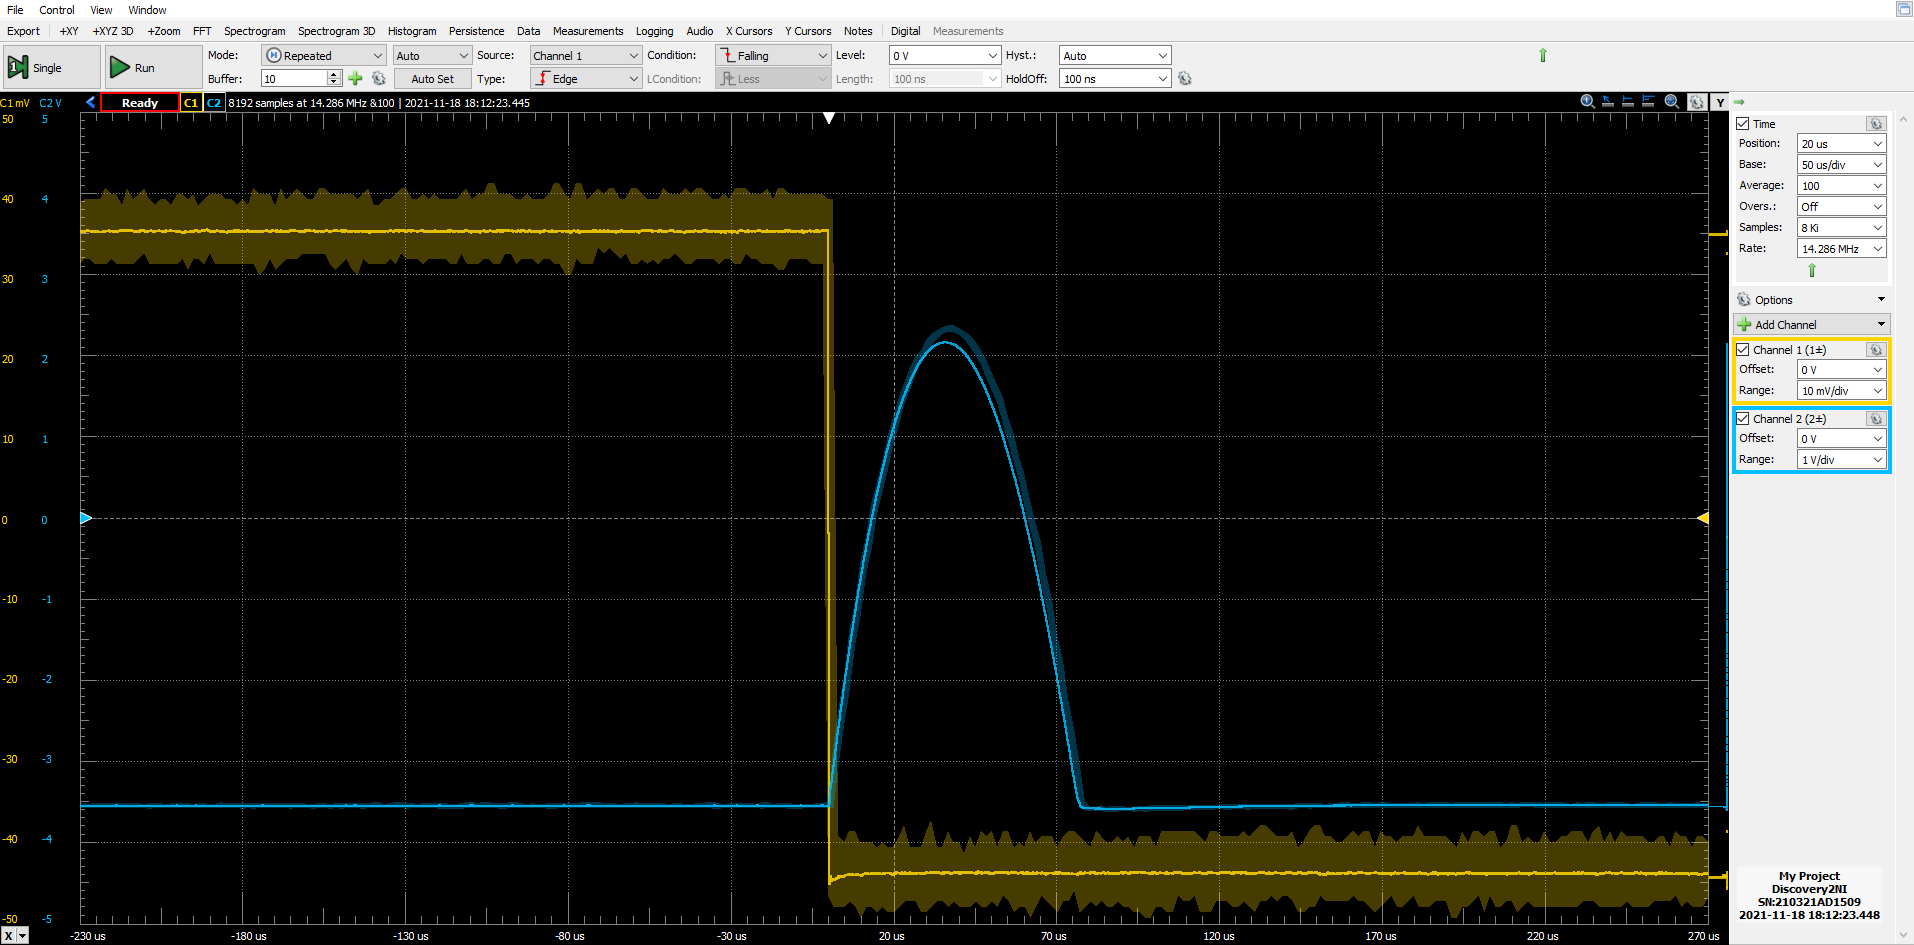
\includegraphics[scale=0.335]{discr_sat}
	\caption{Acquisizione del segnale in uscita dal circuito discriminatore con
	un'onda quadra in ingresso $V_s = \SI{30}{m\V}$, $f = \SI{100}{\Hz}$
	\label{fig: discr_sat}}
\end{figure}

Questo comportamento si osserva fino a circa $\SI{20}{m\V}$, quando il segnale
in uscita dal comparatore non è più apprezzabilmente diverso dalla tensione di
saturazione del trigger.

Il fronte di salita all'uscita del discriminatore è sicuramente limitato dallo
slew-rate finito dell'amplificatore, per cui effettivamente ci aspettiamo
un tempo di salita dell'impulso in ingresso dell'ordine dei
\[
t_{oh} = V\ped{discr}^{pp}/\mathrm{SR} = 7.9 / 13 \approx 0.7 \; \si{\micro\s}
\]
che è in ottimo accordo con quanto si trova da una misura diretta (con i
cursori) della durata del fronte di salita dell'impulso in uscita
$t_{oh} = 717 \pm 10 \; \si{\micro\s}$.

Mentre il fronte di discesa è meno ripido perché corrisponde alla transizione
del discriminatore sulla discesa esponenziale di $V\ped{sh} (t)$, che ha una
derivata ``piccola'' in prossimità della soglia. Questo infatti lascia
presumere che esista un intervallo temporale durante il quale l'uscita di
$V\ped{discr} (t)$ è in regime lineare. Possiamo provare a darne una stima
come il tempo necessario perché l'onda $V\ped{sh} (t)$ decada esponenzialmente
dalla tensione di soglia $V\ped{thr}$ al minimo valore per cui osserviamo un
segnale $V\ped{discr} (t)$ alla tensione di saturazione positiva $V_{OH}$ in
uscita (discussa meglio in \cref{sub: Qmin})
\begin{equation}
t_{ol} = \tau \ln{\left(\frac{V\ped{thr}}{V\ped{min}}\right)} =
35.9 \pm 1.5 \; \si{\micro\s}
\end{equation}
che risulta compatibile con la durata del fronte di discesa dell'onda in
uscita dal discriminatore, misurata anche stavolta con i cursori
$t_{ol} = 36.3 \pm 0.5 \; \si{\micro\s}$.

A testimonianza di questa possibile transizione al regime lineare abbiamo
studiato la forma del segnale in uscita, per ampiezze dell'onda quadra
prossime alla soglia.
\begin{figure}[htbp]
	\centering
	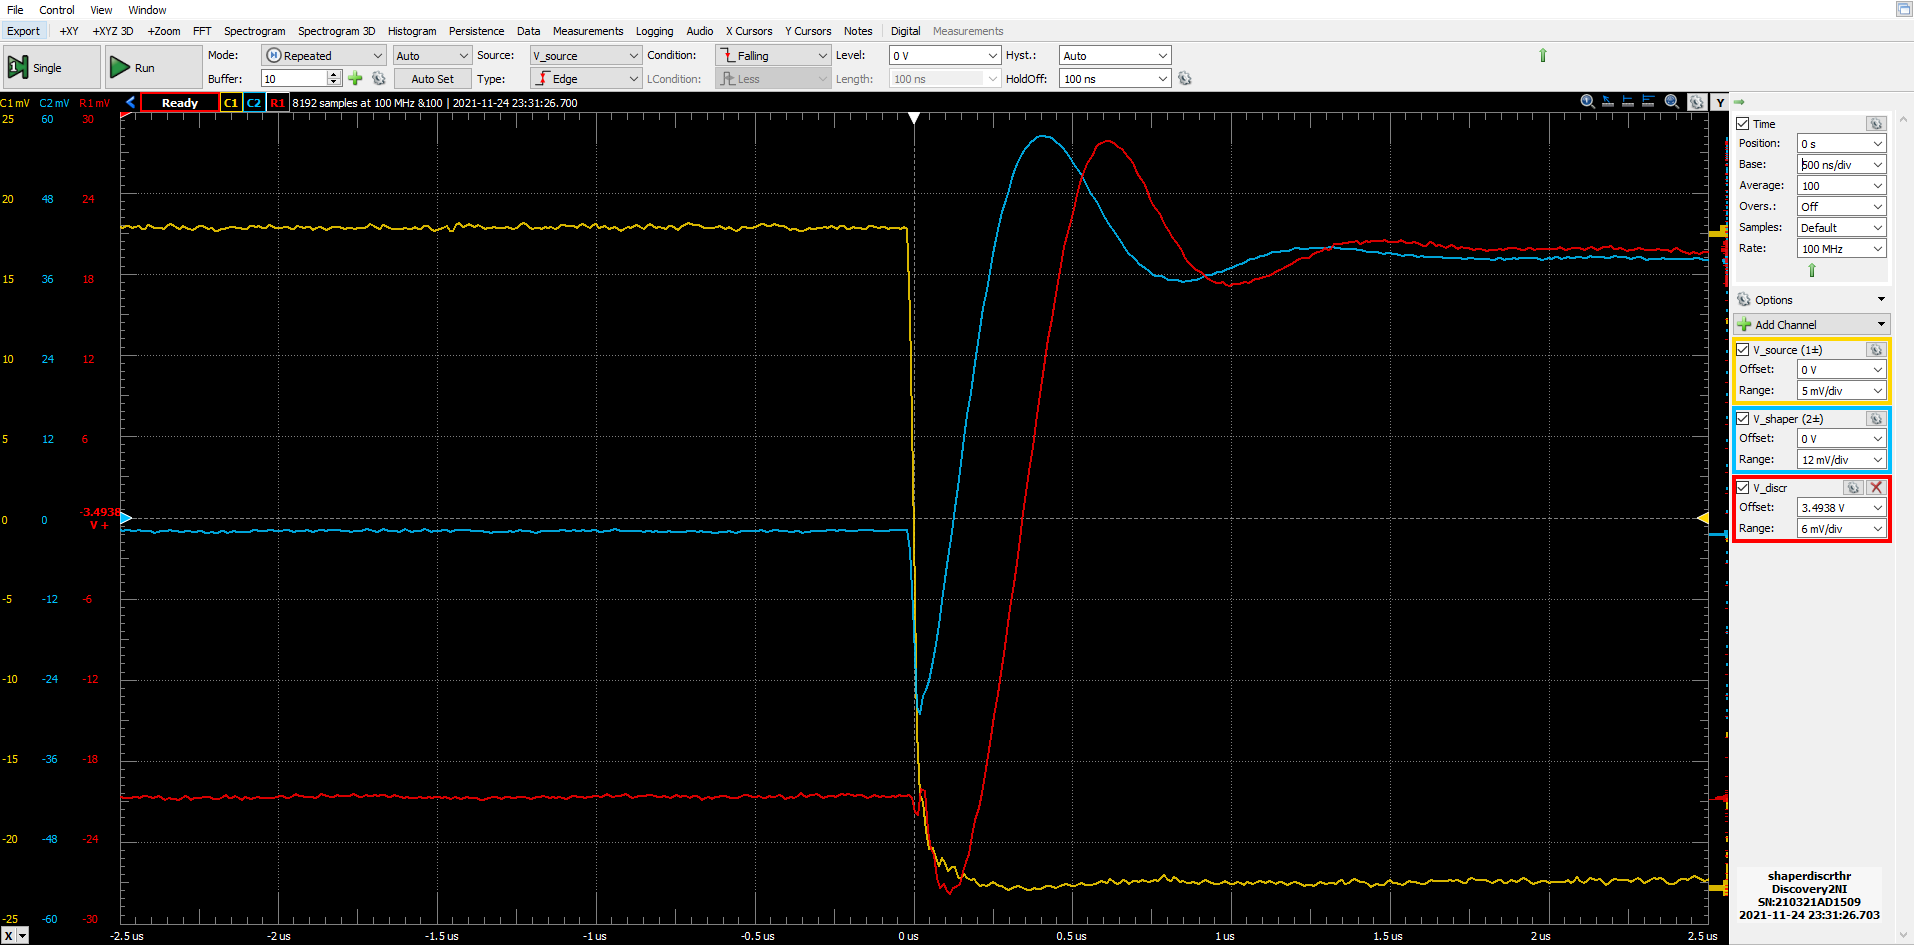
\includegraphics[scale=0.335]{shdiscthr}
	\caption{Acquisizione del segnale in uscita dal circuito discriminatore con
	un'onda quadra in ingresso $V_s = \SI{20}{m\V}$, $f = \SI{100}{\Hz}$
	\label{fig: discrthr}}
\end{figure}
In cui è possibile riconoscere il transiente in uscita dallo shaper visto in
\cref{fig: shzoom} amplificato dal secondo OpAmp in regime lineare.

\subsection{Minima ampiezza di carica per cui si attiva il comparatore}
\label{sub: Qmin}
Per ottenere una misura di ampiezza minima di carica per cui si registra un
segnale che raggiunga la soglia $V_{OH}$ in uscita dal discriminatore abbiamo
variato l'ampiezza del segnale in ingresso $V_s$ dal generatore di forme
d'onda, dunque abbiamo misurato con i cursori l'ampiezza critica trovata per
i due circuiti studiati:
\begin{align*}
V\ped{min} &= 40.5 \pm 0.3 \; \si{m\V} \\ 
V\ped{min} &= 43.6 \pm 0.4 \; \si{m\V}
\end{align*}
che corrispondono alle quantità di carica minima per gli amplificatori di
$Q\ped{min} = C_T \cdot 2V\ped{min} =
\{80, \; 87\} \pm  3 \; \si{\pico\coulomb}$.

\subsection{Confronto con i valori attesi}
Abbiamo eseguito un fit con legge logaritmica per l'andamento delle misure
del Time-over-Threshold al variare dell'ampiezza di carica in ingresso
$Q\ped{in}$, di cui riportiamo i risultati
\begin{figure}[htbp]
    \centering
	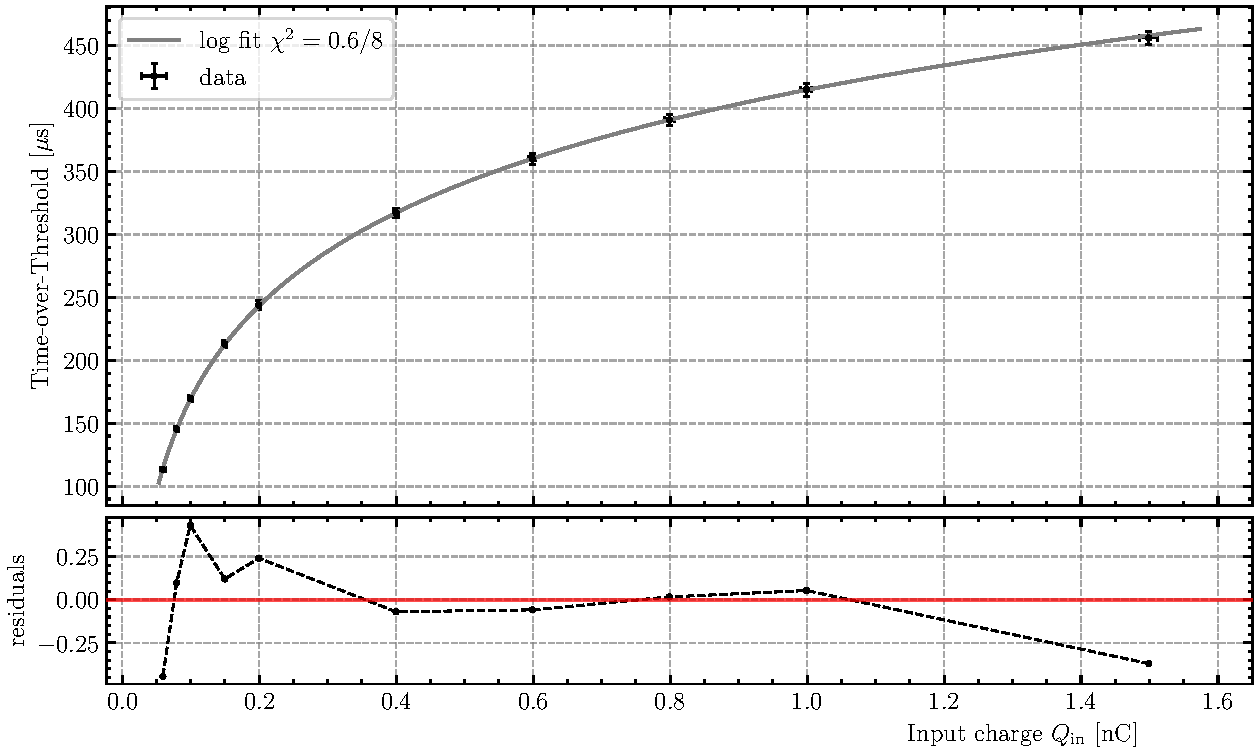
\includegraphics[scale=0.75]{logfit}
    \caption{Fit logaritmico del $ToT$ in funzione dell'ampiezza di carica in
    ingresso $Q\ped{in}$ \label{fig: logfit}}
\end{figure}
\begin{align*}
V\ped{thr} &= 40.7 \pm 0.2 \; \si{m\V}
&\tau = 106.51 \pm 0.3 \; \si{\micro\s} \\
\chi^2/\mathrm{ndof} &= 0.6/8 &\mathrm{cov_{norm}} = 0.82
\end{align*}

Ritroviamo che il valore del tempo di smorzamento $\tau$ è compatibile con il
valore atteso dai componenti del circuito.
e che la tensione di soglia trovata dal fit è compatibile con il valore di
ampiezza del segnale in ingresso $V\ped{min}$ corrispondente alla minima
ampiezza di carica del punto precedente.

%=======================
\section{Trigger di Schmitt}
Abbiamo costruito un trigger di Schmitt o comparatore con isteresi a partire
dall'OpAmp TL081CP come in \cref{fig: trgschmittschm}.
\begin{figure}[htbp]
    \centering
	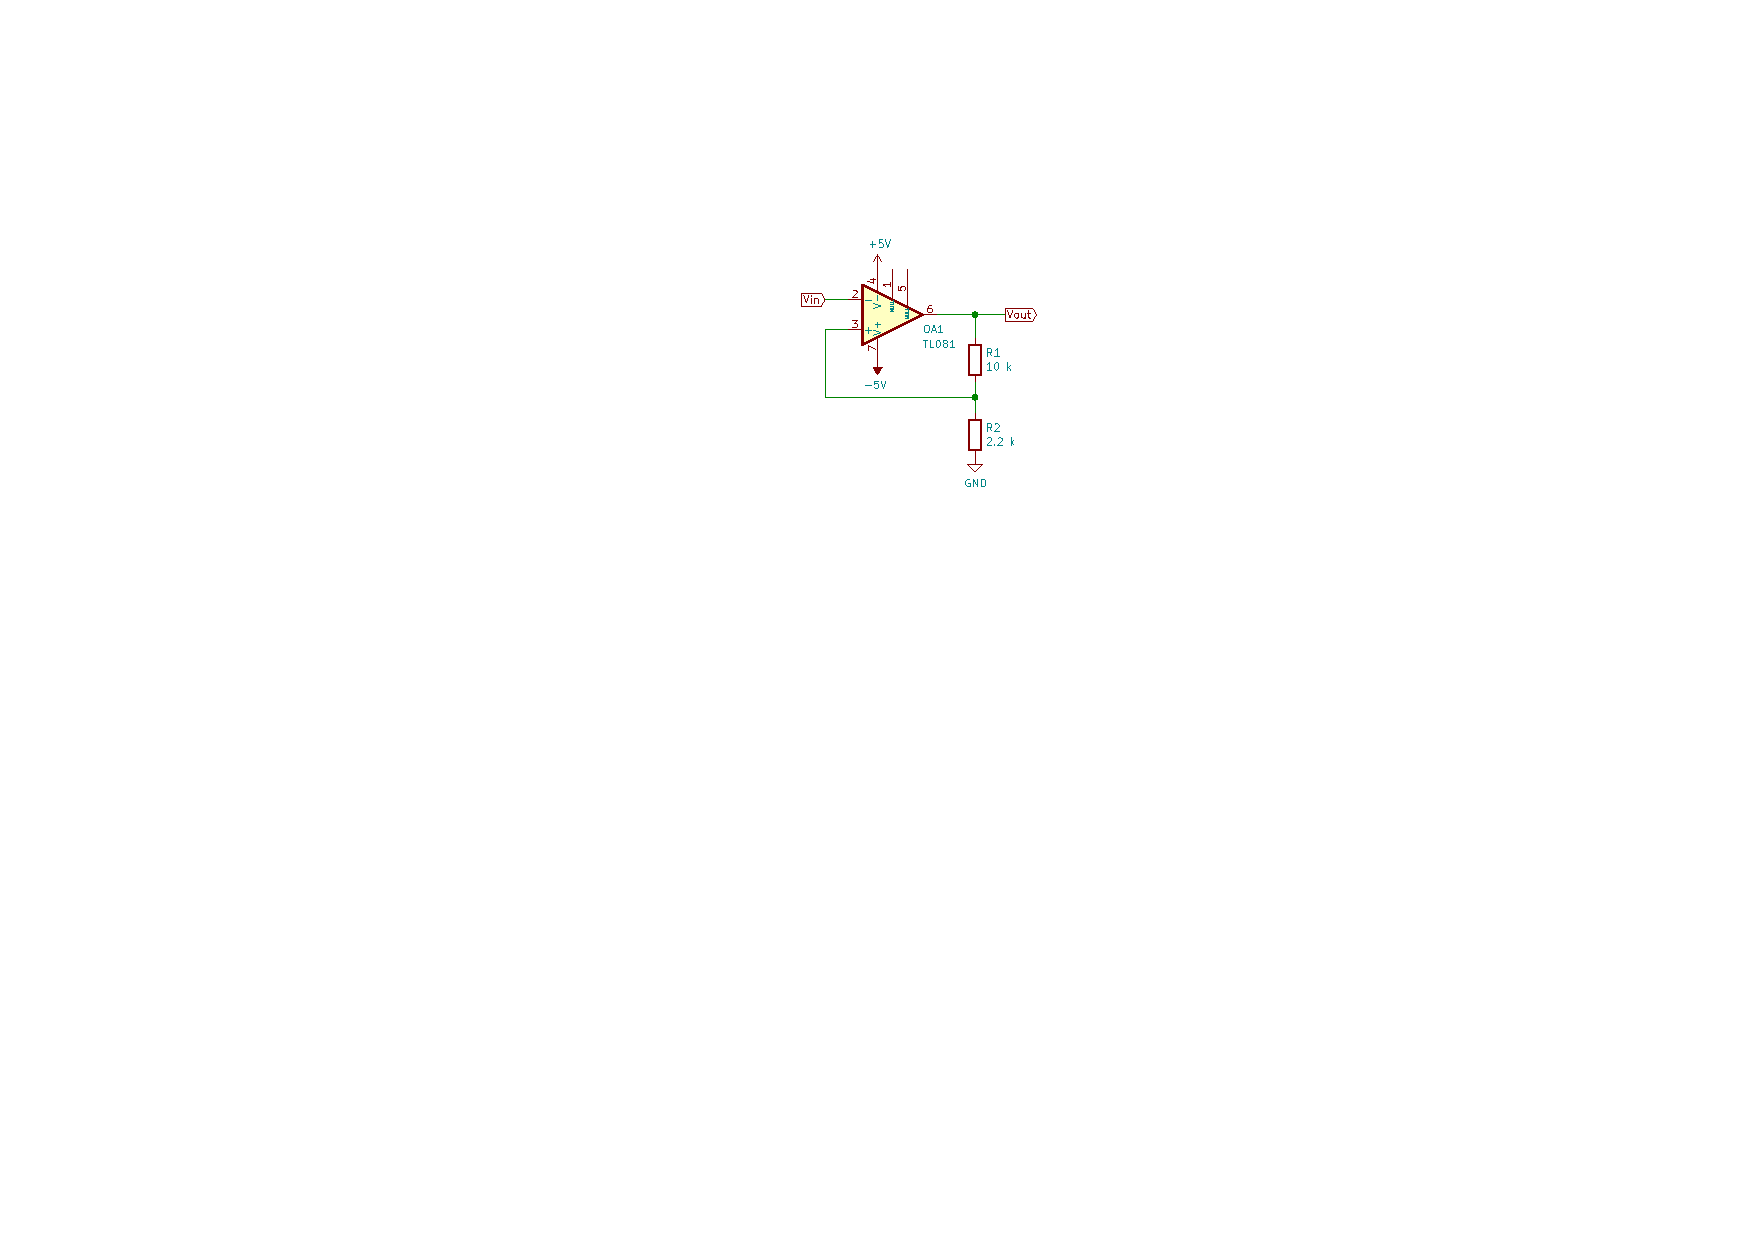
\includegraphics[scale=1.8]{trgSchmitt}
    \caption{Schema circuitale del trigger di Schmitt costruito.
    \label{fig: trgschmittschm}}
\end{figure}

\subsection{Risposta ad un'onda sinusoidale}
Abbiamo inviato all'ingresso invertente dell'OpAmp un'onda sinusoidale di
ampiezza $V_s = 999 \pm 8 \; \si{m\V}$ e frequenza $f = 100.0 \pm 1.6 \; \si{\Hz}$.
Si osserva immediatamente che né le due tensioni di saturazione, né tantomeno
le tensioni di soglia sono uguali in valore assoluto. \`E per questo motivo
che l'onda quadra in uscita dal trigger ha una componente continua positiva,
quindi la sua traccia visualizzata all'oscilloscopio risulta traslata verso
l'alto.
\begin{figure}[htbp]
	\centering
	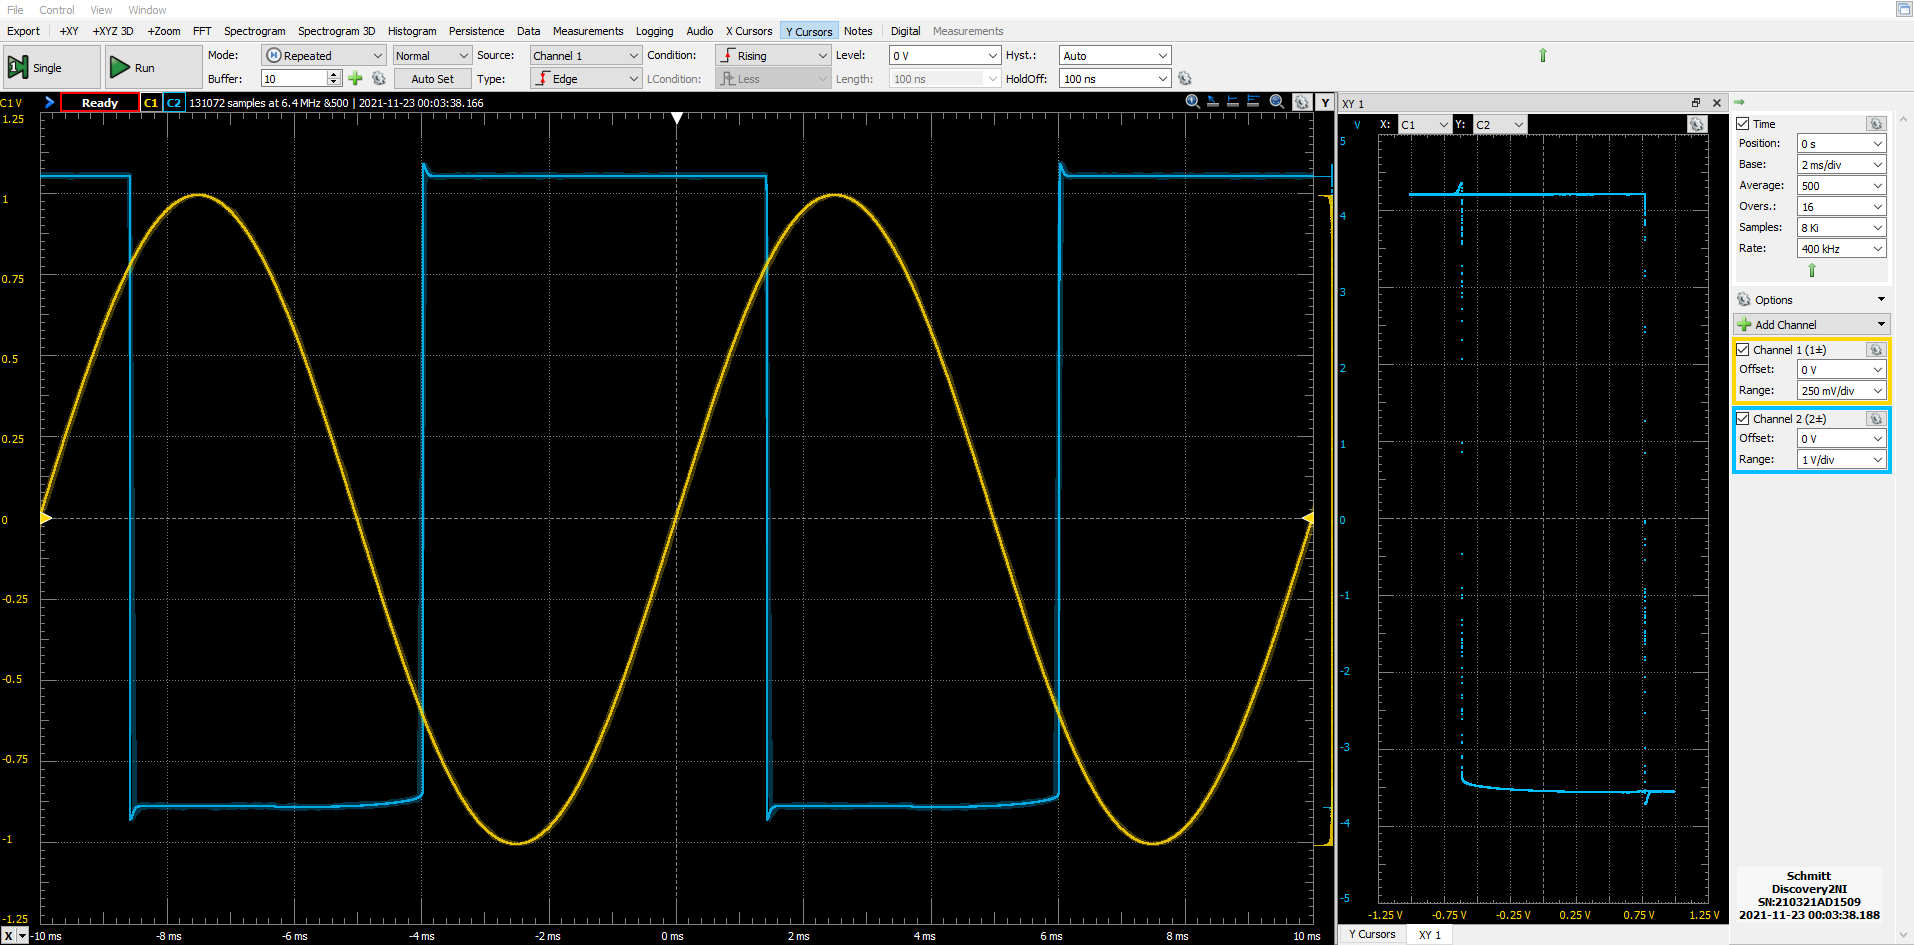
\includegraphics[scale=0.335]{schmitt}
	\caption{Risposta del trigger di Schmitt ad un segnale sinusoidale di ampiezza
	$V_s = \SI{1}{V}$ e frequenza $f = \SI{100}{Hz}$. \label{fig: schmittsine}}
\end{figure}

La stessa asimmetria si riscontra nel grafico XY dei segnali in ingresso e
uscita dal circuito, in cui le 2 rette di transizione verticali corrispondono
ai valori delle tensioni di soglia $V_{TL}$ e $V_{TH}$ del trigger. Queste
non sono simmetriche rispetto a $\SI{0}{V}$, ma risultano traslate verso
destra.
\begin{figure}[htbp]
	\centering
	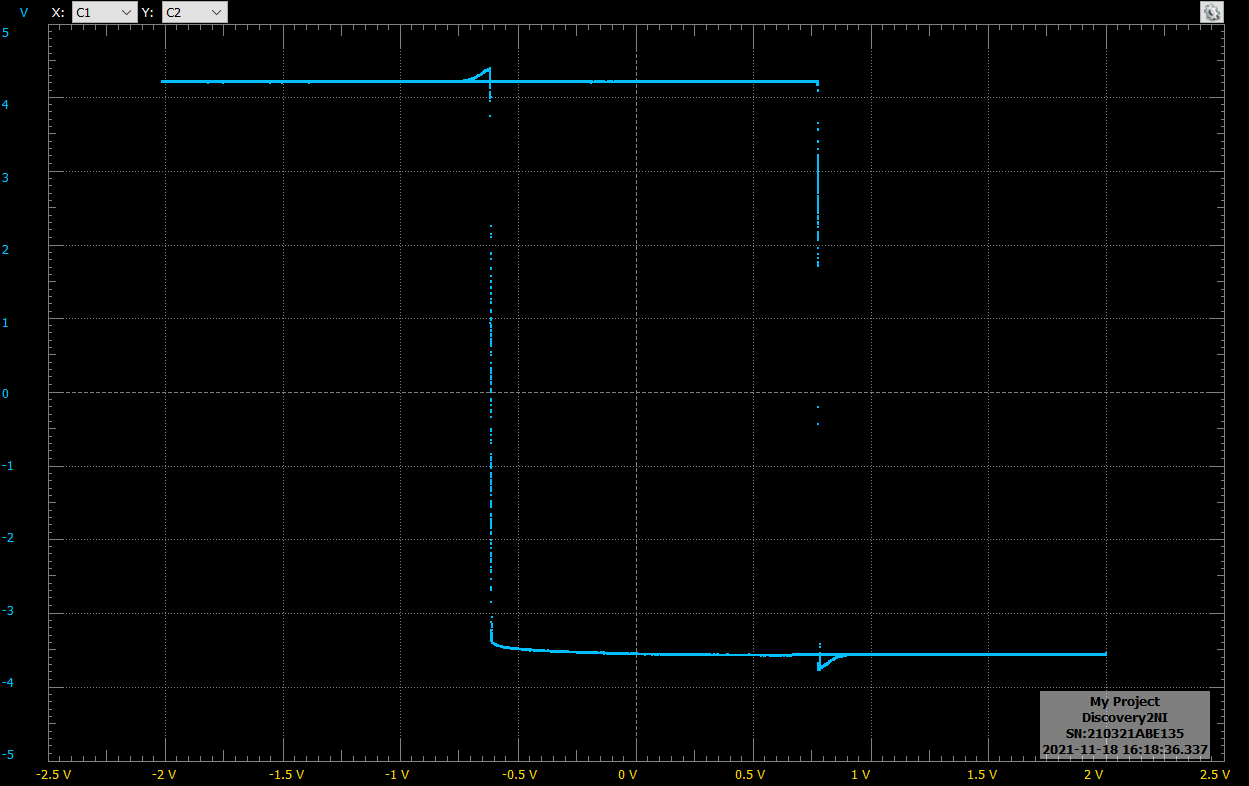
\includegraphics[scale=0.6]{shmitt_isteresi}
	\caption{Visualizzazione XY del seno di ampiezza $V_s = \SI{2}{\V}$ e
	frequenza $\SI{100}{\Hz}$ in ingresso e del segnale in uscita dal trigger di
	Schmitt. \label{fig: schmittxy}}
\end{figure}

\subsection{Saturazione dell'OpAmp}
Abbiamo misurato le tensioni di saturazione dell'OpAmp direttamente
dai valori alto $V_{OH}$ e basso $V_{OL}$ -pressoché costanti- che assume
l'onda quadra in uscita dal trigger tramite i cursori:
\begin{align*}
V_{OH} &= 4.28 \pm 0.04 \; \si{\V} \\
V_{OL} &= -3.66 \pm 0.03 \; \si{\V}
\end{align*}
Per il secondo circuito abbiamo trovato, allo stesso modo
\begin{align*}
V_{OH} &= 4.21 \pm 0.04 \; \si{\V} \\
V_{OL} &= -3.53 \pm 0.03 \; \si{\V}
\end{align*}

\subsection{Tensioni di soglia e funzionamento del trigger}
Ora abbiamo inviato in ingresso al circuito (nonché all'ingresso invertente
dell'OpAmp) un'onda sinusoidale di ampiezza
$1999 \pm 15 \; \si{m\V}$ e frequenza fissata a $1000 \pm 16 \; \si{\Hz}$.

Dalle intersezioni tra i canali in ingresso ed uscita abbiamo misurato le
tensioni per cui si verificano le transizioni basso-alto $V_{TH}$ e alto-basso
$V_{TL}$ nel primo trigger
\begin{align*}
V_{TH} &= -617 \pm 5 \; \si{m\V} \\
V_{TL} &= 775 \pm 6 \; \si{m\V}
\end{align*}
Per il secondo circuito invece abbiamo preso una media pesata dei punti che
giacciono sulle 2 linee verticali che si formano nelle transizioni del ciclo
di isteresi visto nel grafico XY di \cref{fig: schmittxy}.
\begin{align*}
V_{TH} &= -611.6 \pm 0.5 \; \si{m\V} \\
V_{TL} &= 780.4 \pm 0.5 \; \si{m\V}
\end{align*}

Supponiamo che l'OpAmp si comporti come il comparatore/discriminatore già
visto nell'amplificatore di carica, quindi che la differenza
$v_d = v_+ - v_- $ sia abbastanza grande da far sì che si trovi sempre in
regime non lineare. In piena analogia con quanto discusso nella
\cref{sub: discr}, come segnale in uscita dal comparatore ci aspettiamo
\[
V\ped{out} = V_{CC} \sgn(v_+ - v_-)
.\]
Inoltre, dal momento che l'ingresso non-invertente è collegato all'uscita del
partitore di tensione costituito da $R_1$ e $R_2$, abbiamo
\[
v_+ = \frac{R_2}{R_1 + R_2} V \ped{out} = \beta V\ped{out}
\]
dove abbiamo implicitamente definito il coefficiente di partizione
$\beta \coloneqq \frac{R_2}{R_1 + R_2}$. Quindi mettendo tutto insieme
\[
V\ped{out} = V_{CC} \sgn(\beta V\ped{out} - V_s)
.\]

Da cui vediamo che la tensione in uscita dal comparatore sarà al livello
``alto'' (i.e. $V\ped{out} = V_{CC}$) quando $V\ped{out} > V_s/\beta$ e
``basso'' (cioè $V\ped{out} = -V_{CC}$) nel caso complementare
$V\ped{out} < V_s/\beta$. Queste condizioni definiscono le tensioni di soglia
per cui ci aspettiamo avvengano le transizioni:
$V_s = \pm V\ped{trn}$, dove
\begin{equation}
V\ped{trn} = \beta V_{CC} = \frac{V_{CC}}{1 + R_1/R_2} =
0.90 \pm 0.03 \; \si{\V}
\end{equation}

Possiamo spiegare il funzionamento del trigger di Schmitt in termini di
feedback positivo, che ne regola il comportamento tramite il controllo del
segnale in ingresso. Se la tensione $V_s$ è minore di $V_{TH} < \SI{0}{\V}$
il segnale in uscita rimane alto. Al crescere della tensione del segnale
in ingresso fino al valore di soglia
$V_s \geq V_{TL} \implies V\ped{out} \mapsto -V_{CC}$ il segnale in uscita
dal circuito salta repentinamente dal livello alto a basso. Dunque
$V\ped{out}$ rimane basso fintanto che la tensione in ingresso non diminuisce
al di sotto della soglia opposta
$V_s \leq V_{TH} \implies V\ped{out} \mapsto V_{CC}$, per cui il segnale in
uscita sale velocemente al livello alto.

Il che corrisponde esattamente a quanto si riesce ad osservare visualizzando
i segnali in ingresso ed uscita con l'oscilloscopio in \cref{fig: schmittsine}.

\subsection{Limiti fisici del circuito}\label{sub: trglim}
Si osserva che il circuito si comporta come discriminatore con isteresi per
frequenze sufficientemente basse; più precisamente possiamo individuare una
frequenza limite $f_L$, oltre la quale il trigger smette di funzionare.
Il valore di questa frequenza limite dipende anche dall'ampiezza dell'onda che
si invia all'ingresso, per esempio nel caso in cui l'ampiezza sia
$V_s = \SI{1}{\V}$ si trova $f_L \approx 90 \; \si{k\Hz}$, mentre per
$V_s' = \SI{2}{\V}$ la frequenza limite aumenta fino a
$f_L' \approx 700 \si{k\Hz}$. Riportiamo di seguito le misure della frequenza
trovate da uno scan con Network per i due circuiti in queste due
configurazioni:
\begin{align*}
f_L &= 92.6 \pm 0.1 \; \si{k\Hz} \\
f_L' &= 680 \pm 4 \; \si{k\Hz}
\end{align*}

\begin{figure}[htbp]
	\centering
	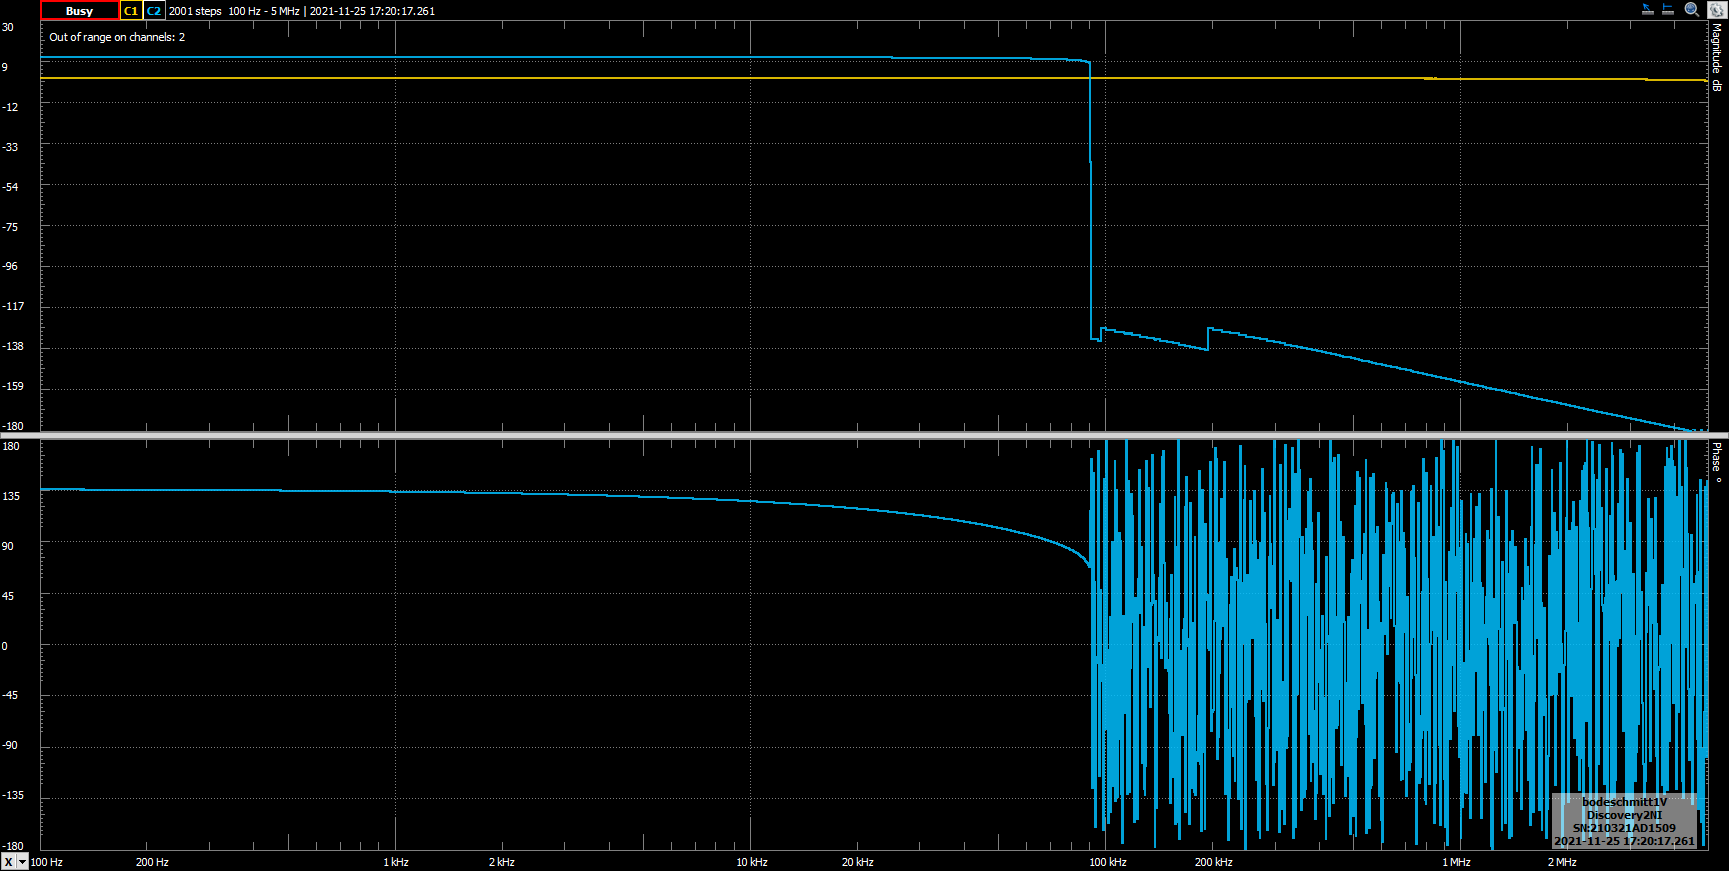
\includegraphics[scale=0.335]{bodeschmitt1V100Hz5MHz}
	\caption{Analisi in frequenza del trigger di Schmitt, con ampiezza del segnale
	in ingresso fissata ad $\SI{1}{V}$, l'unico punto di interesse si trova a
	circa $\SI{90}{k\Hz}$, frequenza oltre alla quale il circuito non ha più
	il comportamento atteso.}
\end{figure}

\begin{figure}[htbp]
	\centering
	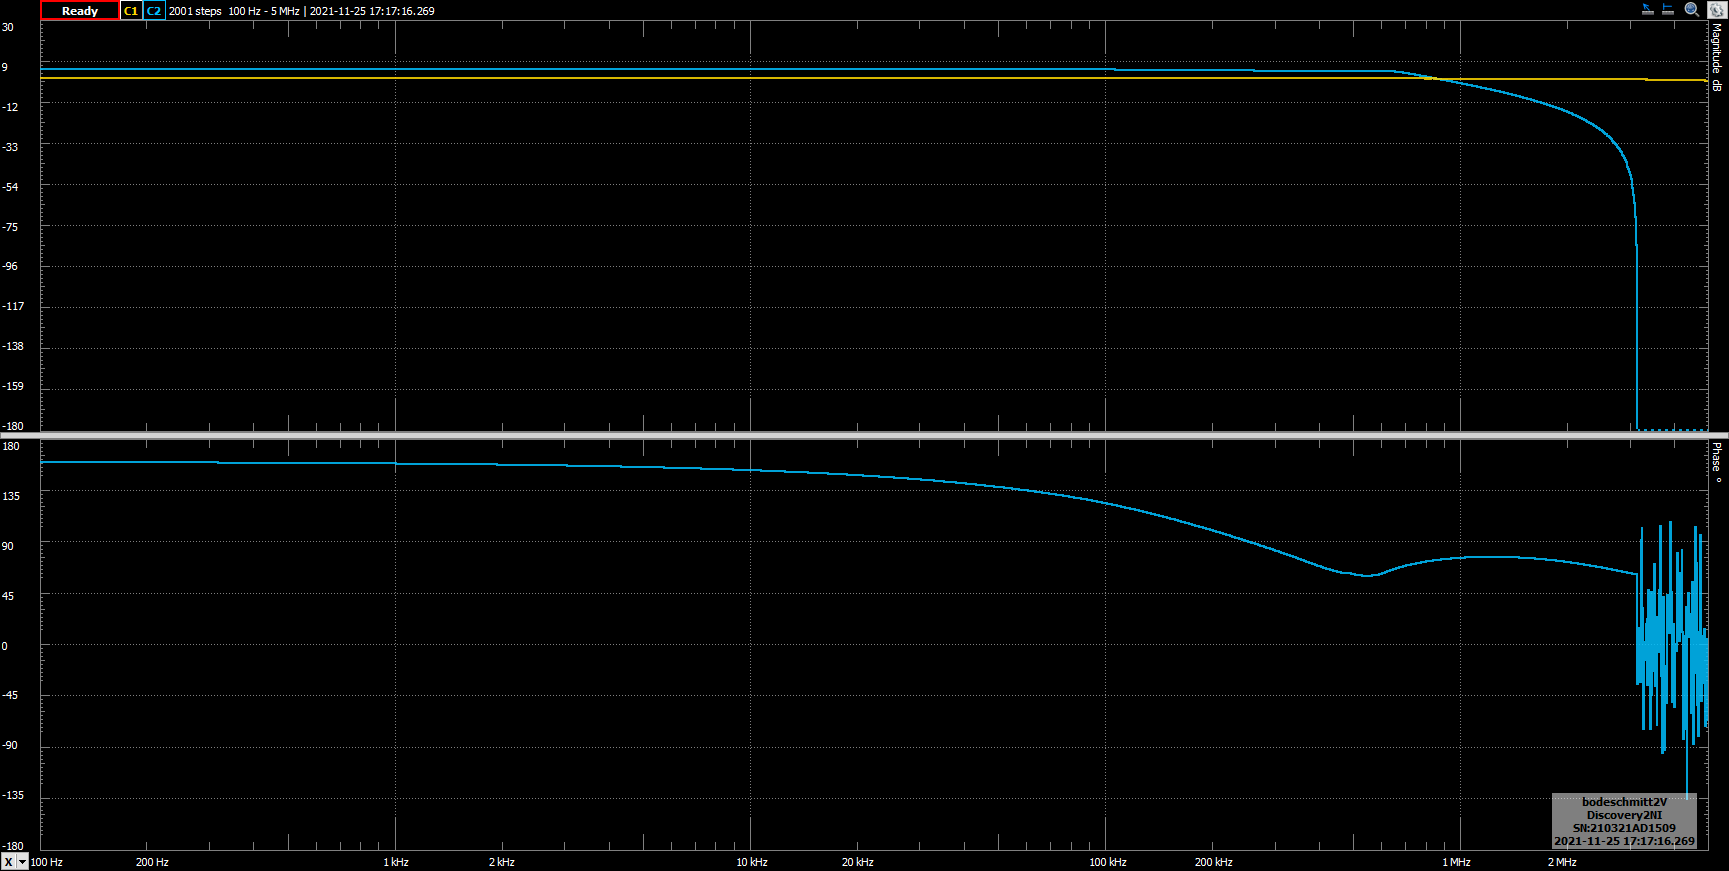
\includegraphics[scale=0.335]{bodeschmitt2V100Hz5MHz}
	\caption{Risposta in frequenza del trigger di Schmitt, con ampiezza del
	segnale in ingresso fissata a $\SI{2}{V}$, a partire dai $\SI{700}{k\Hz}$
	osserviamo una deviazione dall'andamento atteso.}
\end{figure}

Per frequenze maggiori di $\sim \SI{10}{k\Hz}$ la pendenza della transizione
del segnale in uscita da ``alto'' a ``basso'' e viceversa comincia ad essere
limitata dallo slew-rate dell'OpAmp.
Per cui dal fronte d'onda tra le transizioni dello stato del trigger abbiamo
scelto di misurare direttamente lo slew-rate del TL081
\begin{align*}
\mathrm{SR} &= 11.1 \pm 0.3 \; \si{\V/\micro\s} \\
\mathrm{SR} &= 11.3 \pm 0.3 \; \si{\V/\micro\s}
\end{align*}

Effettivamente, affinché l'OpAmp possa funzionare correttamente come
discriminatore con isteresi, occorre che il tempo minimo di salita e discesa
siano molto minori rispetto al periodo dei segnali in ingresso e in uscita:
\begin{equation}\label{eq: slewlim}
T \gg 2 t\ped{min}, \qquad t\ped{min} =
\frac{V\ped{out}^{pp}}{\mathrm{SR}} \approx \SI{0.7}{\micro\s}
\implies \frac{1}{T} = f \ll \SI{700}{k\Hz}.
\end{equation}
che risulta in accordo con quanto si è trovato sperimentalmente.

Variando l'ampiezza del segnale in ingresso $V_s$ si osserva che l'ampiezza del
segnale in uscita rimane pressoché uguale a $V\ped{out}^{pp} = V_{OH} - V_{OL}
= 7.94 \pm 0.04$ fino a una soglia inferiore intorno a $\SI{800}{m\V}$, al di
sotto della quale l'uscita è costante al valore di saturazione $V_{OH}$.
Infatti per quanto abbiamo visto, affinché il circuito possa compiere il ciclo
di isteresi, l'ampiezza (picco-picco) del segnale in ingresso deve essere
maggiore della base del rettangolo di isteresi $V_s^{pp} \geq 2 V\ped{trn}$.
In realtà, per via dell'asimmetria delle tensioni di soglia, è necessario
che $V_s$ abbia ampiezza superiore alla soglia $V_{TL}$, in modulo la
più alta delle due; come si è visto dall'esperimento.

Notiamo infine che al diminuire dell'ampiezza dell'onda in ingresso (a partire
dal massimo valore generabile di $V\ped{s, max} = \SI{5}{\V}$ fino a soglia
$V_s \approx V_{TL} \approx \SI{800}{m\V}$)
corrispondono un aumento della componente continua (da un minimo di circa
$560 \; \si{m\V}$ ad un massimo valore registrato di $1.5 \; \si{\V}$) e del
duty cycle (a partire da un valore minimo di $50.6 \pm 1.1 \%$ fino a
$65.6 \pm 1.2 \%$ per valori di $V_s$ molto vicini alla soglia) nell'onda
quadra in uscita dal circuito.

%=======================
\section{Multivibratore astabile}
Il circuito in \cref{fig: astableschm} è costituito da un trigger di
Schmitt con un filtro passa-basso RC collegato all'ingresso invertente dell'
OpAmp.
\begin{figure}[htbp]
    \centering
	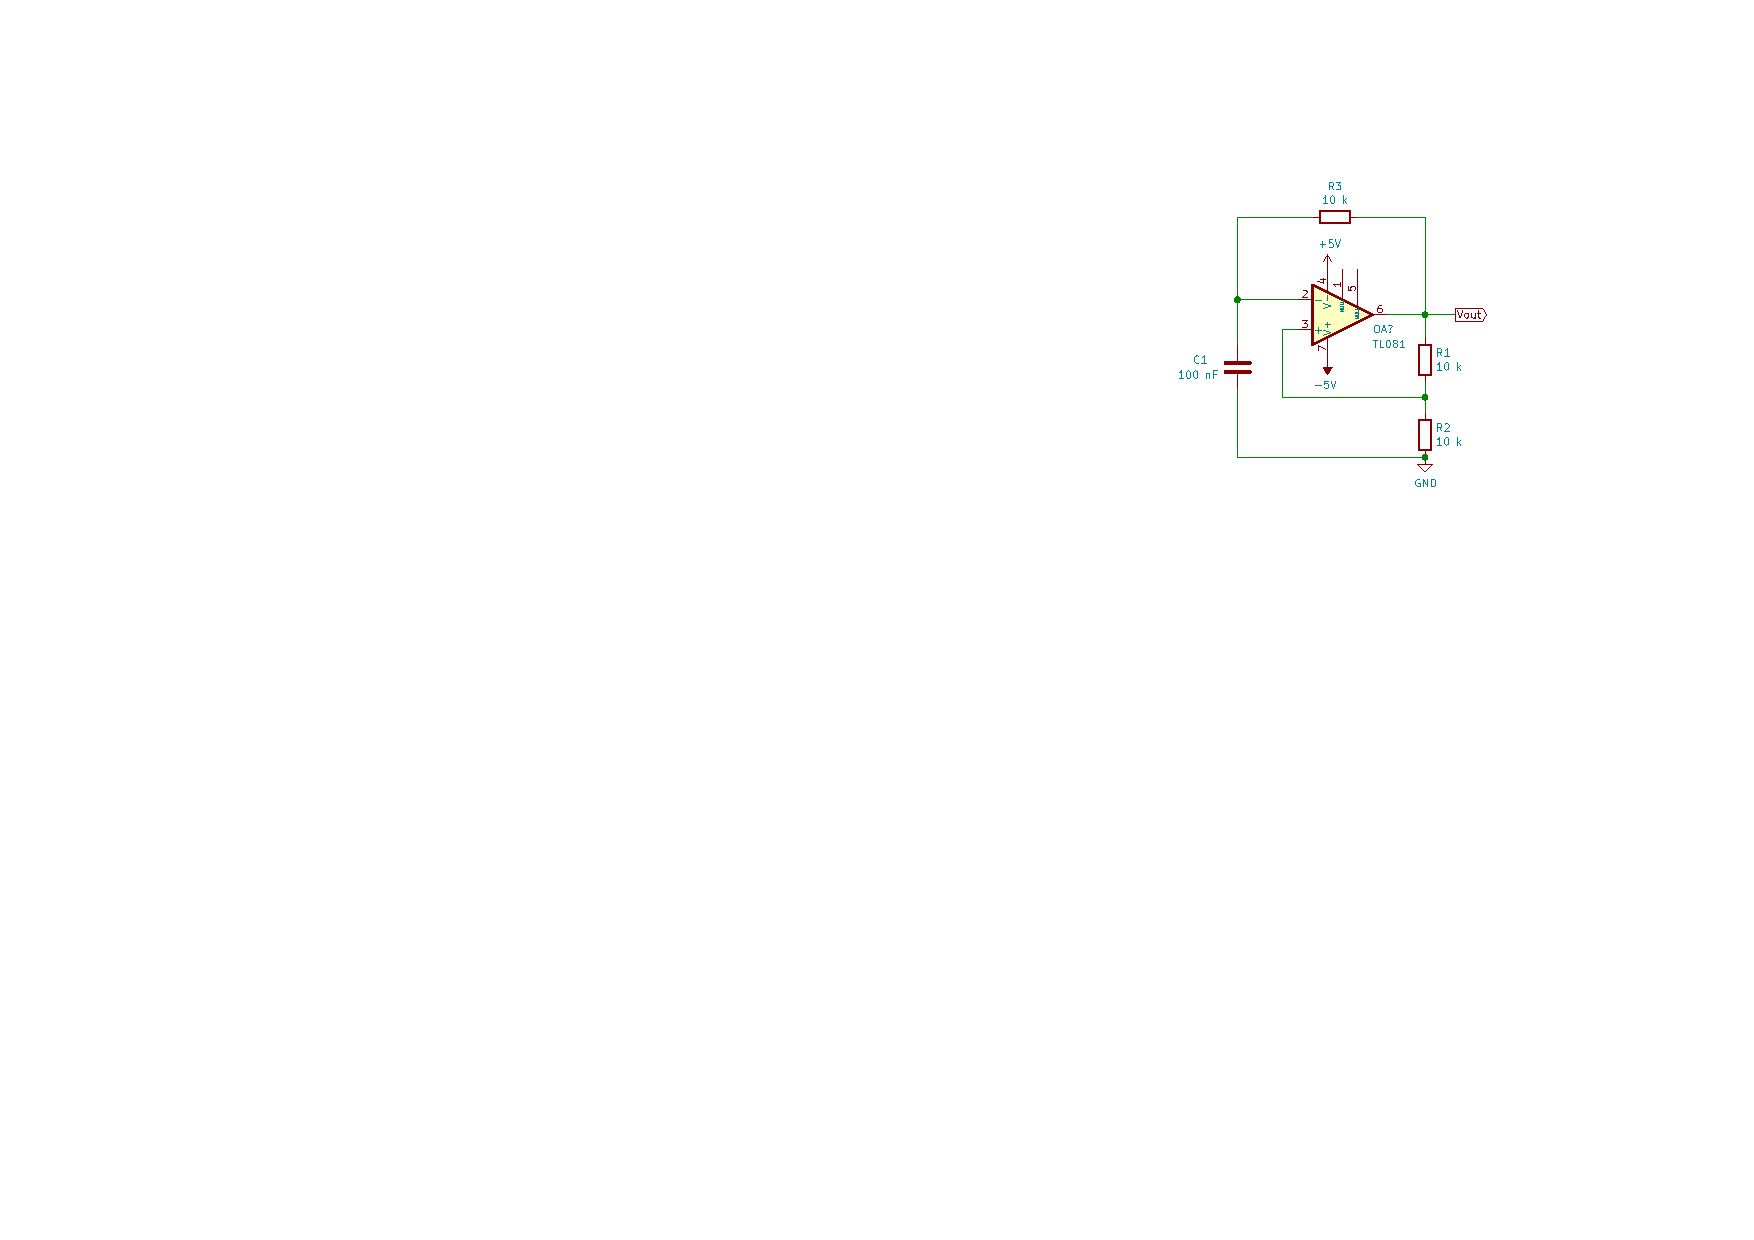
\includegraphics[scale=1.5]{astable}
    \caption{Schema circuitale del multivibratore astabile costruito.
    \label{fig: astableschm}}
\end{figure}

\subsection{Funzionamento del circuito}
Per spiegarne il funzionamento è fondamentale studiare il comportamento del
condensatore collegato all'ingresso negativo dell'OpAmp $C_1$. Questo si
carica fino a raggiungere la stessa d.d.p. al terminale positivo
dell'operazionale, a questo punto il trigger cambia rapidamente stato da alto
a basso e, di conseguenza, la tensione all'ingresso non-invertente si abbassa.
Dunque il condensatore comincia a scaricarsi fino a che la d.d.p. ai suoi capi
non raggiunge la stessa tensione ora presente all'ingresso non invertente
dell'amplificatore operazionale.
Il ciclo quindi si ripete generando un'onda quadra in uscita, il cui
periodo di oscillazione è proporzionale al doppio del tempo caratteristico
$\tau = R_3 C_1$ in cui il condensatore è in grado di caricarsi/scaricarsi.

Più precisamente, una volta definite
\begin{align*}
q &= \frac{R_2}{R_1 + R_2} = 0.502 \pm 0.003 \\
\tau &= R_3 C_1 = 95 \pm 4 \; \si{\micro\s}
\end{align*}
Abbiamo come valori attesi per i tempi caratteristici alto $t_H$ e basso
$t_L$ ed il periodo $T$ dell'onda quadra generata dal multivibratore:
\begin{align}
t_H &= \tau \ln\left(\frac{1 - q\frac{V_{OL}}{V_{OH}}}{1-q}\right) =
1.04 \pm 0.04 \; \si{m\s} \\
t_L &= \tau \ln\left(\frac{1 - q\frac{V_{OH}}{V_{OL}}}{1-q}\right) =
1.16 \pm 0.05 \; \si{m\s} \\
\end{align}
Conseguentemente il valore del periodo e duty-cycle atteso valgono:
\begin{align}
T &= t_H + t_L = 2.20 \pm 0.06 \; \si{m\s} \\
\mathrm{dc} &= \frac{t_H}{T} = 47 \pm 2 \; \%
\end{align}

\setcounter{subsection}{2}
\subsection{Studio dei segnali in ingresso e uscita}
Osservando il segnale in uscita $V\ped{out} (t)$ ci si aspetta di trovare
un'onda quadra di ampiezza picco-picco $\sim \SI{8}{\V}$, periodo
$T = 2.15 \pm 0.03 \; \si{m\s}$ e duty-cycle $50 \%$. Effettivamente come
tensioni di saturazione alta $V_{OH}$ e bassa $V_{OL}$ dell'onda si è misurato
\begin{align*}
\begin{cases}
V_{OH} &= 4.18 \pm 0.04 \; \si{\V} \\
V_{OL} &= -3.47 \pm 0.03 \; \si{\V}  \implies V\ped{out}^{pp} = 7.65 \pm 0.05
\end{cases}
\end{align*}

Mentre come $v_+ (t)$ ci aspettiamo un'onda della stessa forma di
$V\ped{out} (t)$, ma ridotta in ampiezza di un fattore di partizione
$q \approx 0.5$. Questo corrisponde all'andamento osservato di questi due
segnali, che riportiamo in \cref{fig: v+vout}
\begin{figure}[htbp]
	\centering
	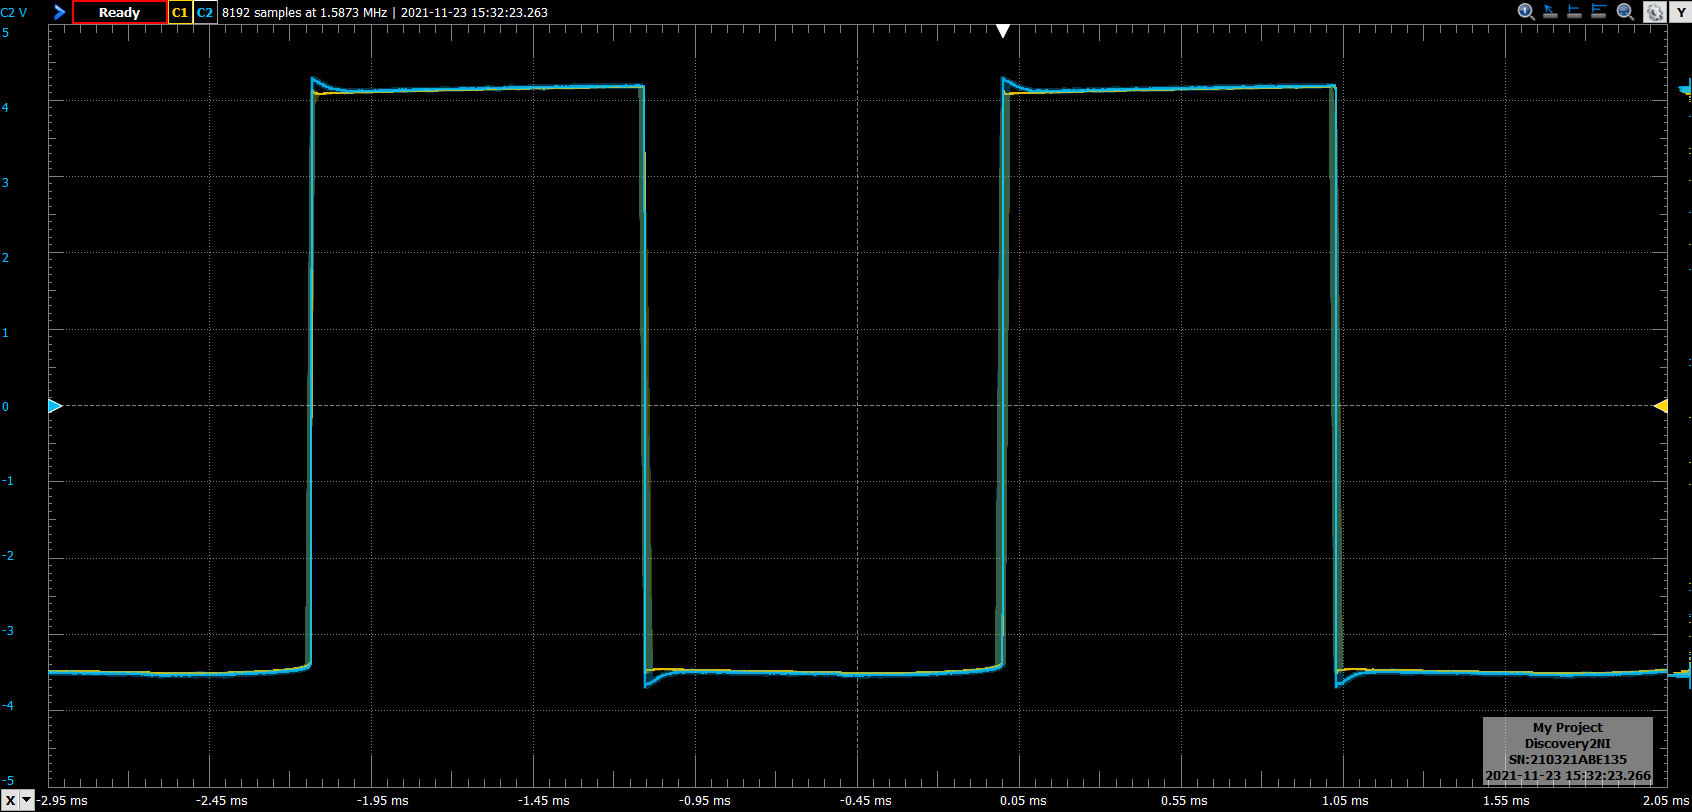
\includegraphics[scale=0.4]{V+Vout}
	\caption{Fermo immagine preso dall'oscilloscopio dell'andamento nel tempo dei
	segnali $v_+ (t)$ (CH1) e $V\ped{out} (t)$ (CH2). \label{fig: v+vout}}
\end{figure}

Osservando $v_- (t)$, infine, ci si aspetta di vedere un segnale ``a pinna di
squalo'', caratteristico del processo di carica/scarica del condensatore e
con la stessa ampiezza di $v_+ (t)$, data dalle tensioni di transizione per
il comparatore/trigger di Schmitt, come riportato in \cref{fig: v-vout}.
\begin{figure}[htbp]
	\centering
	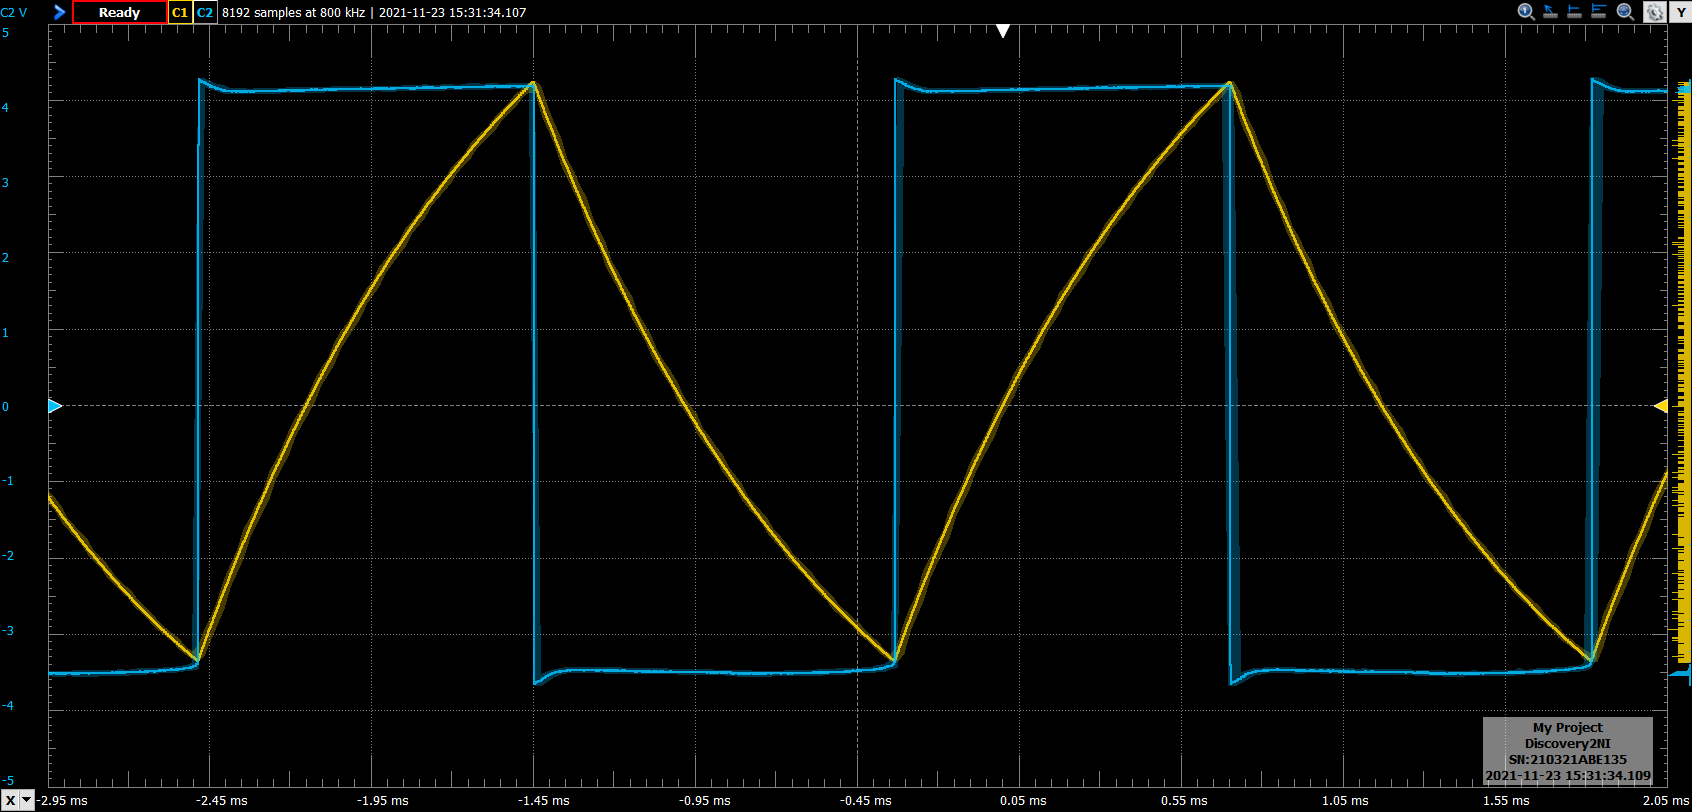
\includegraphics[scale=0.4]{V-Vout}
	\caption{Fermo immagine preso dall'oscilloscopio dell'andamento nel tempo dei
	segnali $v_- (t)$ (CH1) e $V\ped{out}$ (CH2). \label{fig: v-vout}}
\end{figure}

\subsection{Misure di periodo e duty cycle}
Per misurare il periodo dell'onda quadra $V\ped{out} (t)$ e la durata dei
tempi in cui è in saturazione positiva $t_H$ (e negativa $t_L$) si è fatto
uso dei cursori sull'asse X:
\begin{align*}
t_H &= 1.03 \pm 0.02 \; \si{m\s} &\quad t_H &= 1.00 \pm 0.02 \; \si{m\s} \\
t_L &= 1.12 \pm 0.02 \; \si{m\s} &\quad t_L &= 1.08 \pm 0.02 \; \si{m\s} \\
T &= 2.14 \pm 0.01 \; \si{m\s}  &\quad T &= 2.09 \pm 0.16 \; \si{m\s} \\
\end{align*}
Da queste abbiamo ricavato la nostra miglior stima del duty-cycle dell'onda
quadra generata dal multivibratore
\begin{align*}
\mathrm{dc} = \frac{t_H}{T} = 47.9 \pm 1.0 \; \% \\
\mathrm{dc} = \frac{t_H}{T} = 48.2 \pm 0.9 \; \% \\
\end{align*}
Le misure dei tempi in saturazione positiva, negativa e del periodo dei
segnali studiati risultano compatibili con i loro valori attesi, per cui
lo è anche il duty cycle.

\subsection{Limite massimo in frequenza del generatore}
Secondo il nostro modello il periodo dell'onda quadra generata è direttamente
proporzionale a (e anche dello stesso ordine di) $\tau = R_3 C_1$, per cui
se ne vogliamo aumentare la frequenza sarà sufficiente ridurre il valore
della resistenza $R_3$ o della capacità $C_1$. Effettivamente abbiamo osservato
un aumento di un fattore $10$ nella frequenza del treno d'impulsi generato,
a seguito di una riduzione di $C_1$ ed $R_3$ dello stesso fattore, in accordo
con quanto ci si aspetta di vedere per una decimazione del tempo caratteristico
di carica/scarica $\tau$.

L'aumento della massima frequenza generabile non è però l'unico effetto che
si osserva per via della modifica di $\tau$: l'onda quadra in uscita risulta
distorta, specialmente intorno ai fronti di salita e discesa che sono
visibilmente limitati in pendenza, come si vede in \cref{fig: astable1nF}.
\begin{figure}[htbp]
	\centering
	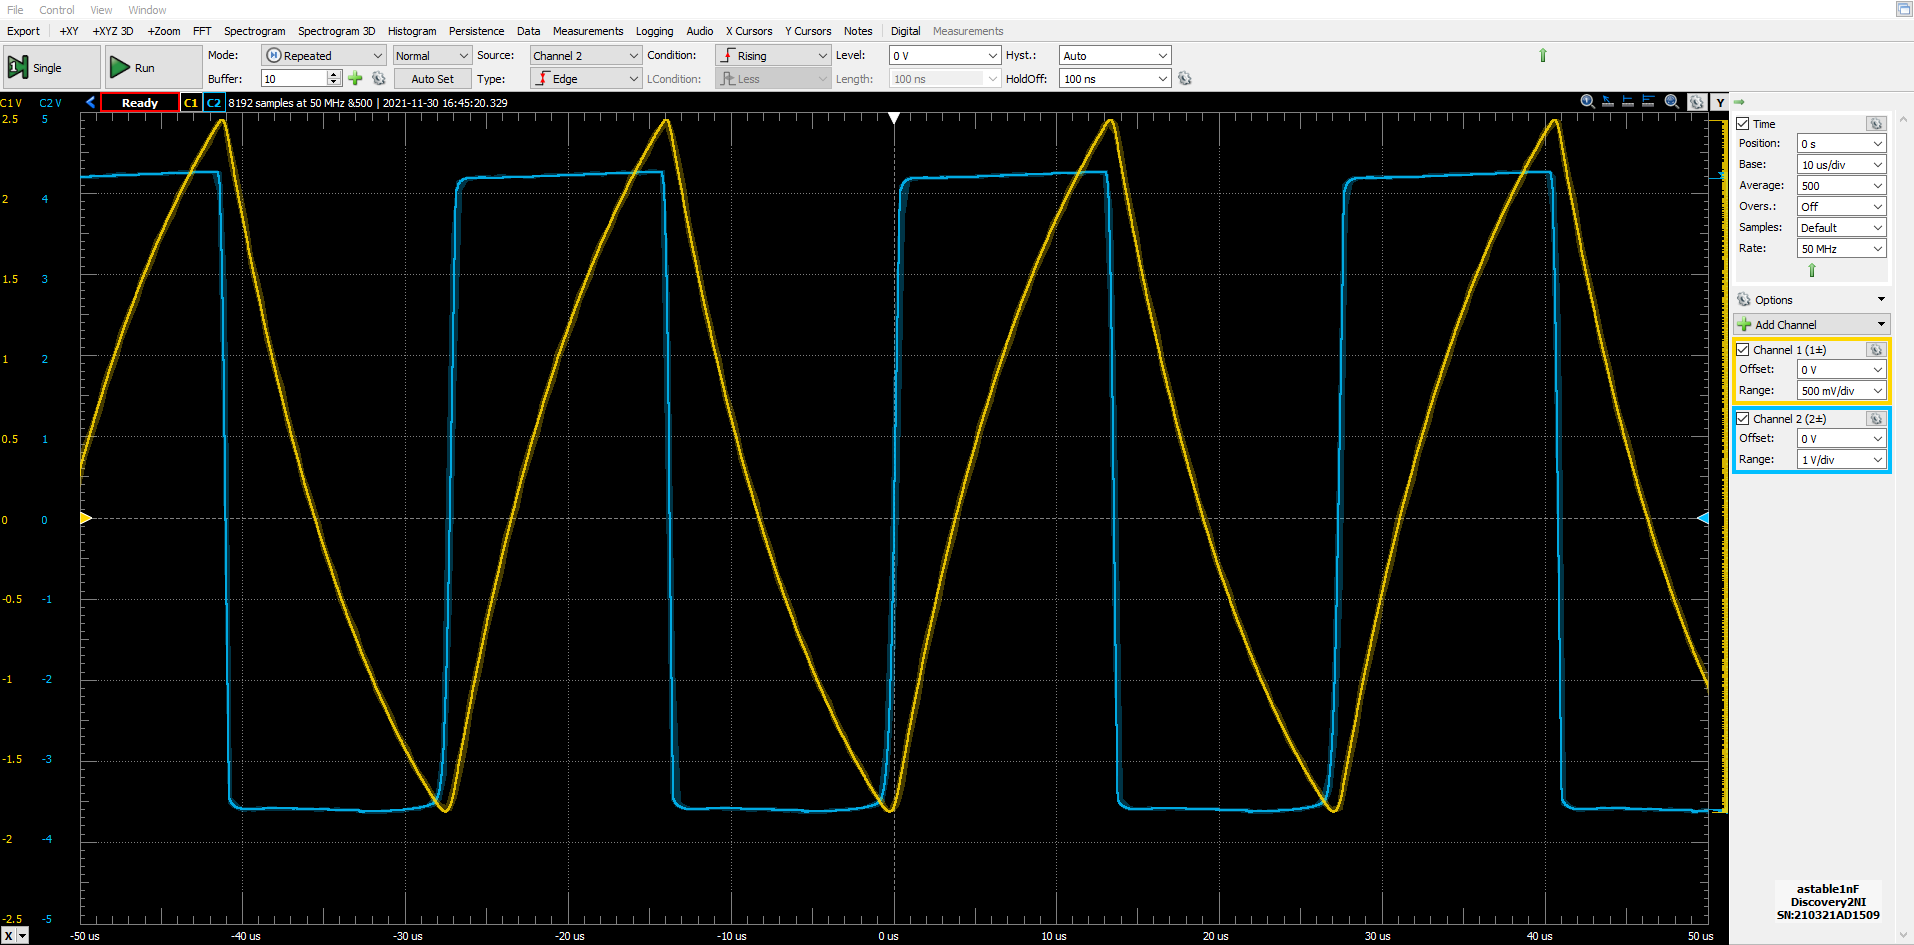
\includegraphics[scale=0.335]{astable1nF}
	\caption{Fermo immagine preso dall'oscilloscopio dell'andamento nel tempo dei
	segnali $v_- (t)$ (CH1) e $V\ped{out} (t)$ (CH2) quando il periodo dell'onda
	generata $T \sim \tau \approx 36 \; \si{\micro\s}$ è ridotto di un fattore di
	circa 10 rispetto alla configurazione originale del circuito.
	\label{fig: astable1nF}}
\end{figure}

In piena analogia con quanto visto nella \cref{sub: trglim}, quando il
semi-periodo dell'uscita si avvicina all'ordine dei $\si{\micro\s}$, cioè il
tempo minimo che l'OpAmp reale impiega per le transizioni di stato dell'onda
quadra di ampiezza picco-picco $V\ped{out}^{pp} \sim \SI{8}{\V}$, il segnale
in uscita presenta fronti di salita e discesa limitati dallo slew-rate
dell'OpAmp, che non riesce a passare abbastanza rapidamente da uno stato
all'altro.

Per verificare che l'effetto di distorsione predominante sia dovuto allo
slew-rate dell'OpAmp, come per il trigger di Schmitt abbiamo misurato (con
i cursori) dalla pendenza dei fronti di salita dell'onda in uscita
$\mathrm{SR} = 11.2 \pm 0.3 \si{V/s}$. Questo è compatibile con l'intervallo
di valori tipici riportato nel datasheet
($\rm SR_{min} = \SI{8}{\V/\micro\s} - SR_{typ} = 13 \; \si{\V/\micro\s}$)
in particolare ci aspettiamo che l'onda quadra generata inizi ad essere
distorta per valori del periodo dell'onda prossimi a
$T\ped{min} \approx 1.4 \; \si{\micro\s}$, compatibilmente con quanto abbiamo
osservato.

Riducendo ulteriormente i valori di resistenza e capacità
($R_3 \approx 220 \; \si{\ohm}$, $C_1 \approx 1 \; \si{nF}$) si osservano
deviazioni ancora più pronunciate dall'onda quadra attesa in uscita, che
possono essere dovute al fatto che il TL081 ha guadagno finito e dipendente
dalla frequenza di lavoro, a differenza di quanto presuppone il nostro modello. 
\begin{figure}[htbp]
	\centering
	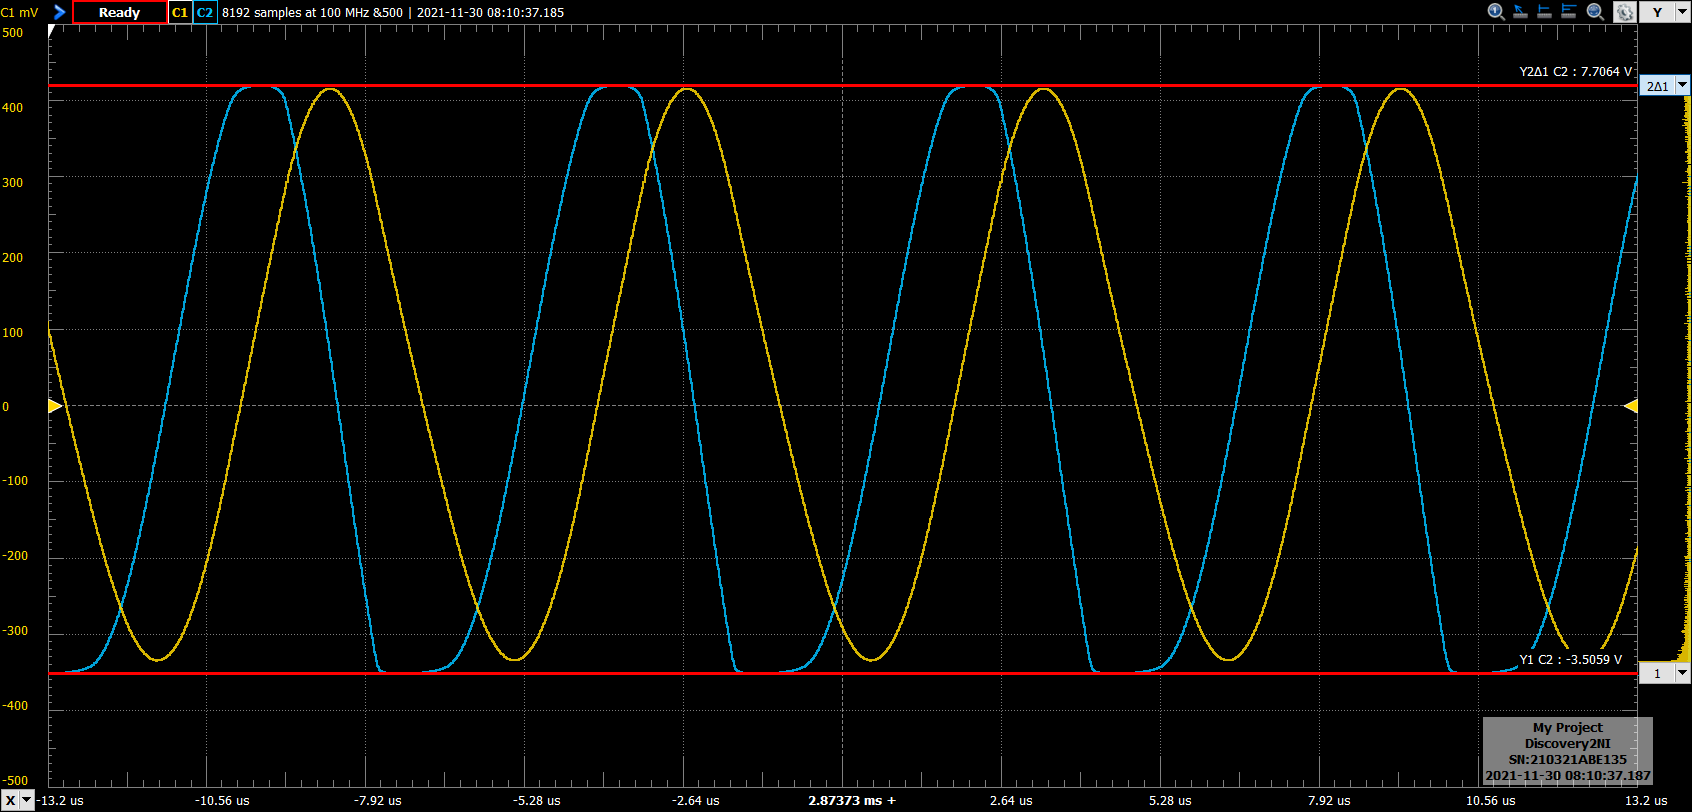
\includegraphics[scale=0.45]{astable(C=1 nF, R= 220 ohm)}
	\caption{Fermo immagine preso dall'oscilloscopio dell'andamento nel tempo dei
	segnali $v_- (t)$ (CH1) e $V\ped{out} (t)$ (CH2) quando il periodo dell'onda
	generata $T \approx \SI{4}{\micro\s}$ è prossimo ai limiti possibili per il
	circuito. \label{fig: astable_lim}}
\end{figure}

%=======================
\section{Multivibratore monostabile}
Il multivibratore monostabile riportato in \cref{fig: mstableschm} è simile
al circuito precedente, ma ha uno stato stabile (quello alto) e uno instabile,
per cui viene utilizzato come generatore di impulsi. In effetti si è costruito
il circuito a partire dallo stesso trigger di Schmitt invertente, aggiungendo
però un sotto-circuito di trigger all'ingresso positivo dell'OpAmp e il diodo
$D_1$ in parallelo al condensatore $C_1$ del filtro passa-basso.
\begin{figure}[htbp]
    \centering
	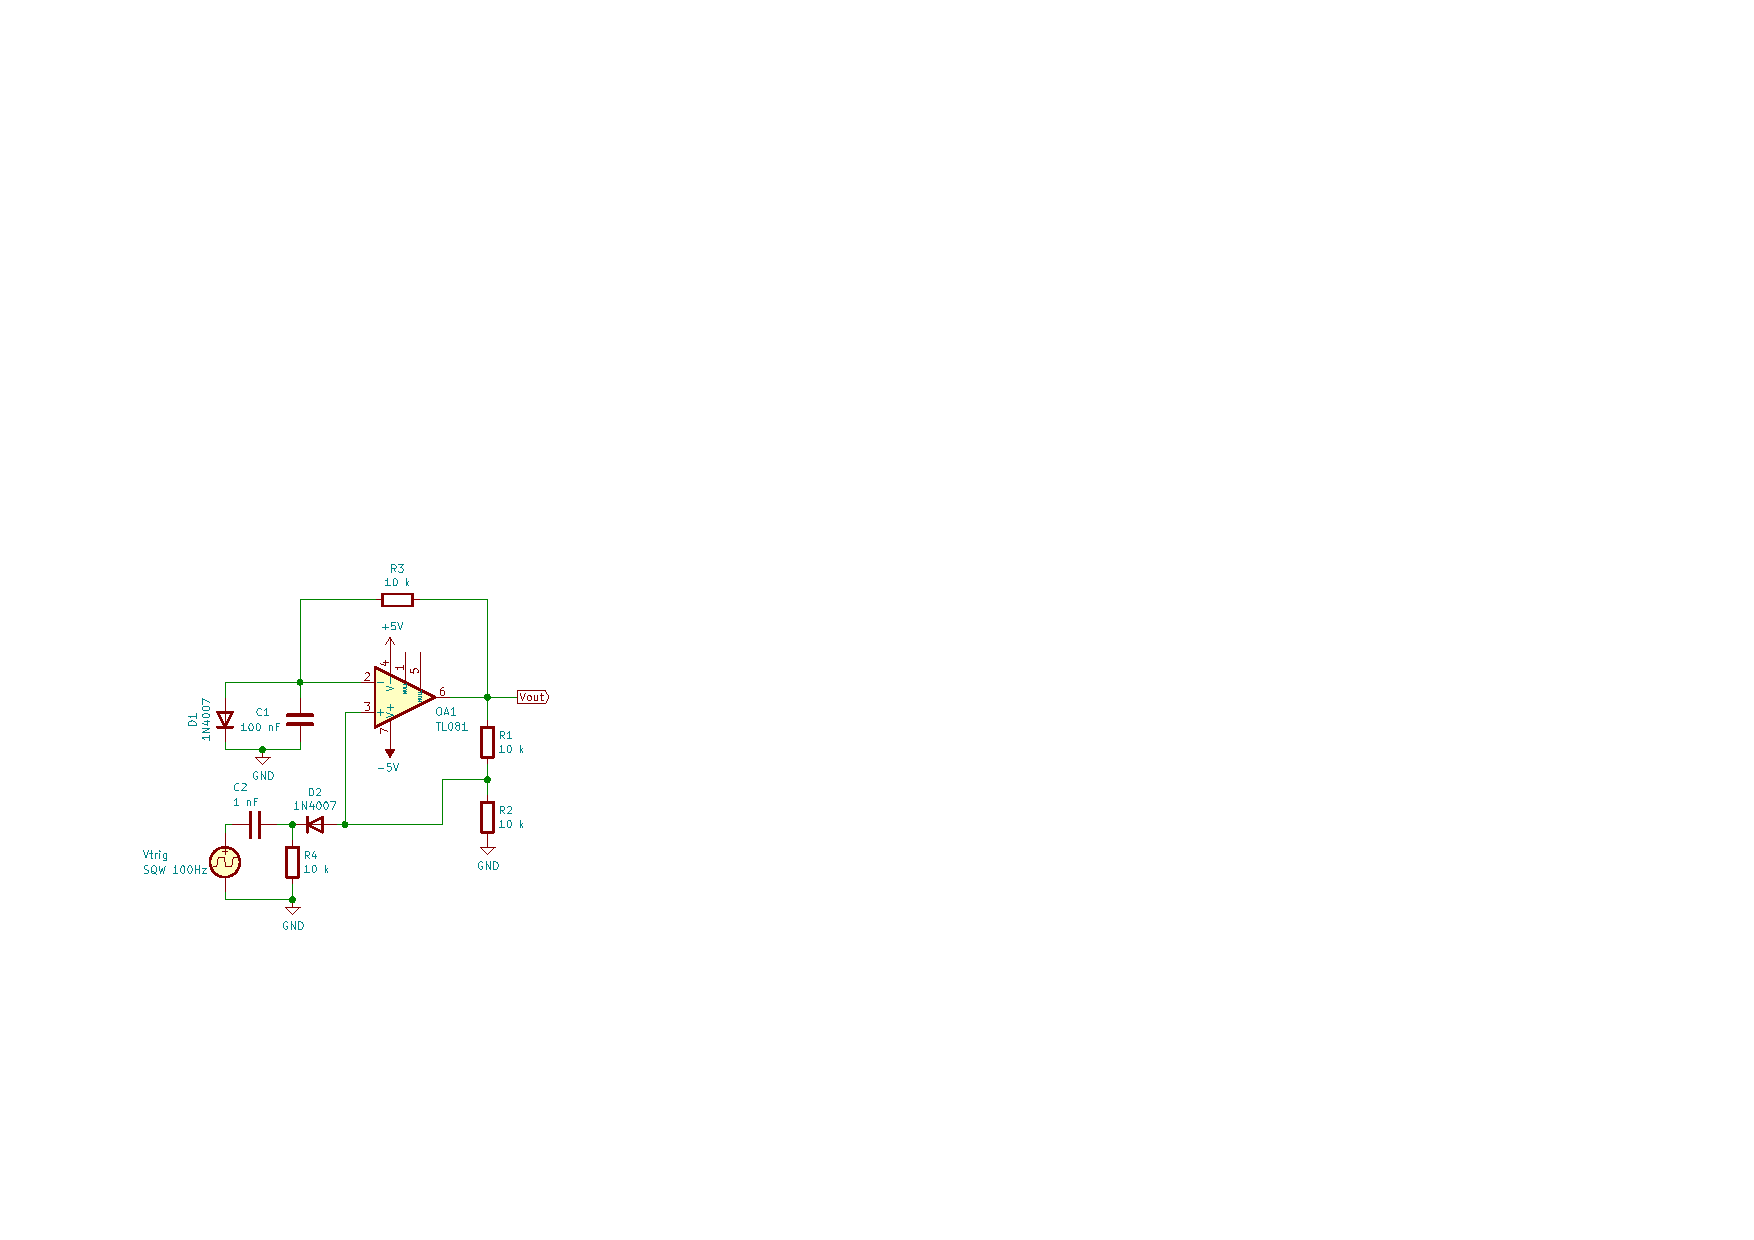
\includegraphics[scale=1.2]{monostable}
    \caption{Schema circuitale del multivibratore monostabile costruito.
    \label{fig: mstableschm}}
\end{figure}

\subsection{Studio dei segnali in ingresso e uscita}
La presenza del diodo in parallelo al condensatore $C_1$ limita la tensione
ai suoi capi $V_C = v_-$, per cui ci aspettiamo di avere
$V_C \leq V\gamma \approx 0.7 \; \si{\V}$, come si trova effettivamente in
\cref{fig: mstabilev-}.
\begin{figure}[htbp]
	\centering
	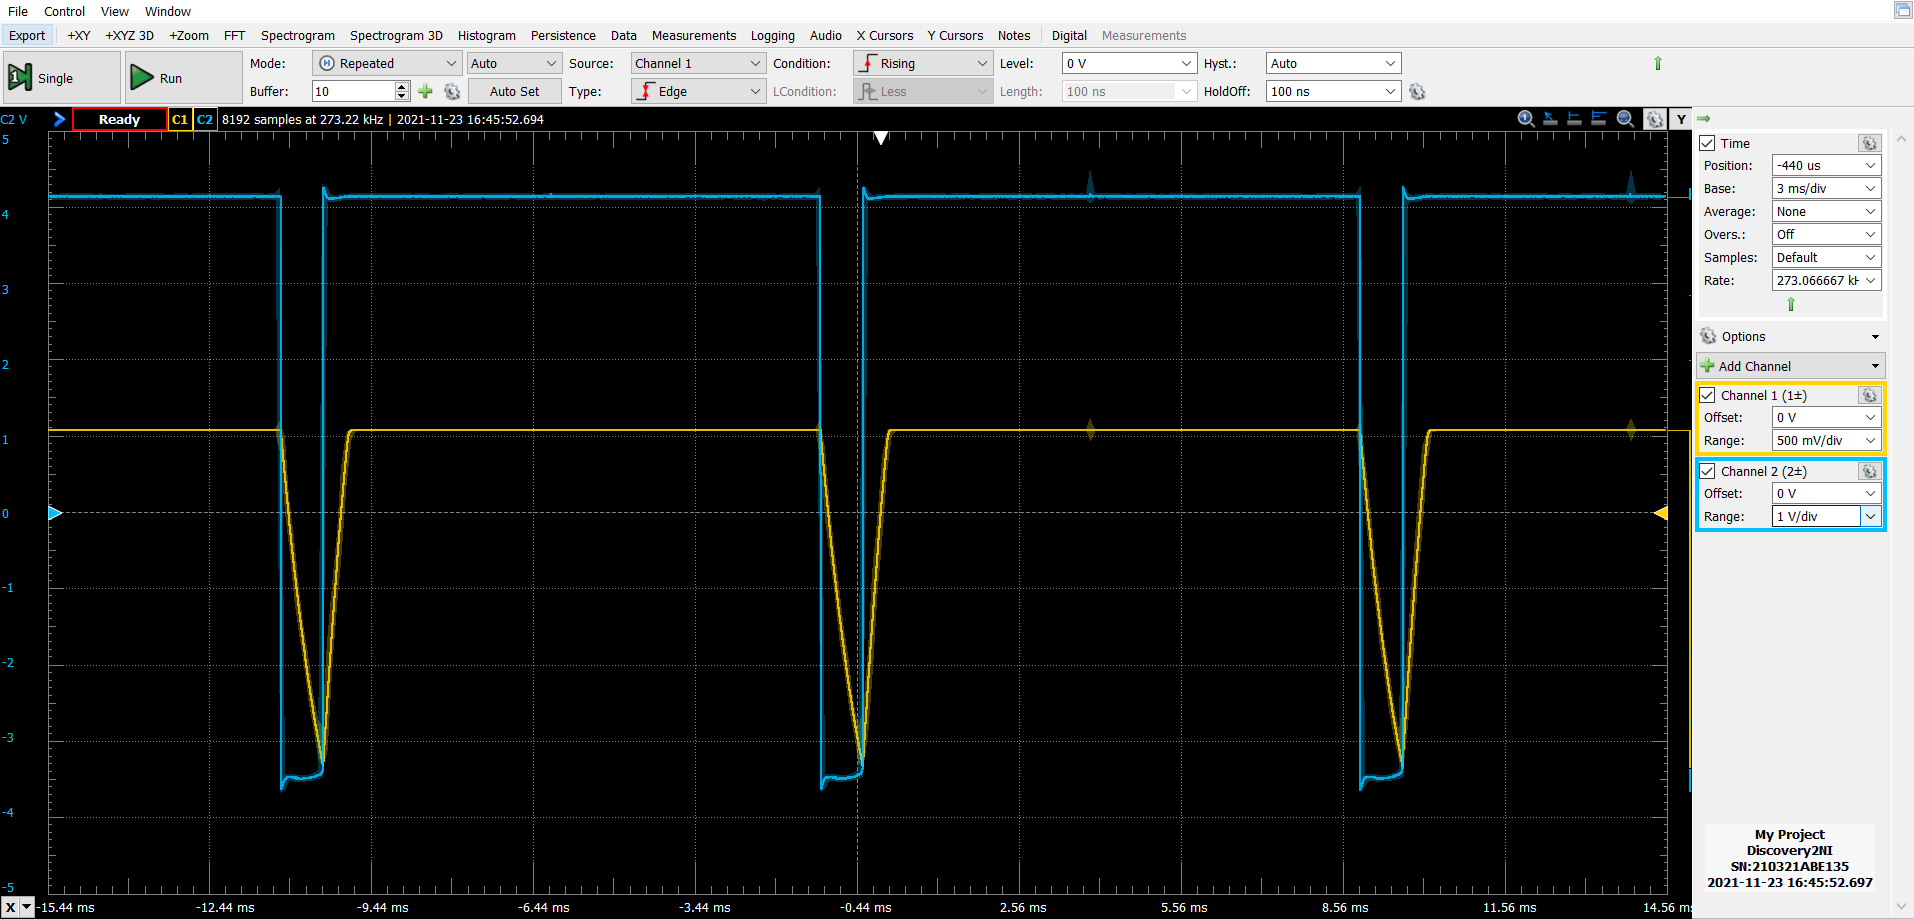
\includegraphics[scale=0.42]{monostabileV-}
	\caption{Acquisizione all'oscilloscopio dell'andamento nel tempo dei
	segnali $v_- (t)$ (CH1) e $V\ped{out} (t)$ (CH2). \label{fig: mstabilev-}}
\end{figure}

\`E per questo che lo stato con l'uscita a livello alto è stabile,
cioè da quest'ultimo il sistema non passa spontaneamente allo stato instabile;
quello con uscita a livello basso.
Dunque per innescare la transizione di stato
$V\ped{out} = V_{OH} \mapsto V_{OL}$ è necessario un circuito di trigger,
che faccia abbassare $v_+$ al di sotto di $v_- \sim V_\gamma$.

In assenza di $V\ped{trig}$, come per il multivibratore astabile, all'ingresso
non-invertente dell'OpAmp ci aspettiamo di trovare come segnale $v_+ (t)$ la
stessa forma d'onda presente all'uscita, ma ridotta in ampiezza di un fattore di partizione $q = \dfrac{R_2}{R_2 + R_1} \approx 0.5$.
Ora però a questa si sovrappongono i picchi di differenza di potenziale che
portano il circuito nello stato instabile sopra descritto; dopo un tempo
caratteristico (proporzionale a $\tau = R_3 C_1$) il multivibratore torna
nella configurazione stabile, generando così un treno di impulsi
negativi/un'onda quadra con duty-cycle prossimo a uno.
Questo è in linea con quanto si vede in \cref{fig: mstabilev+}.
\begin{figure}[htbp]
	\centering
	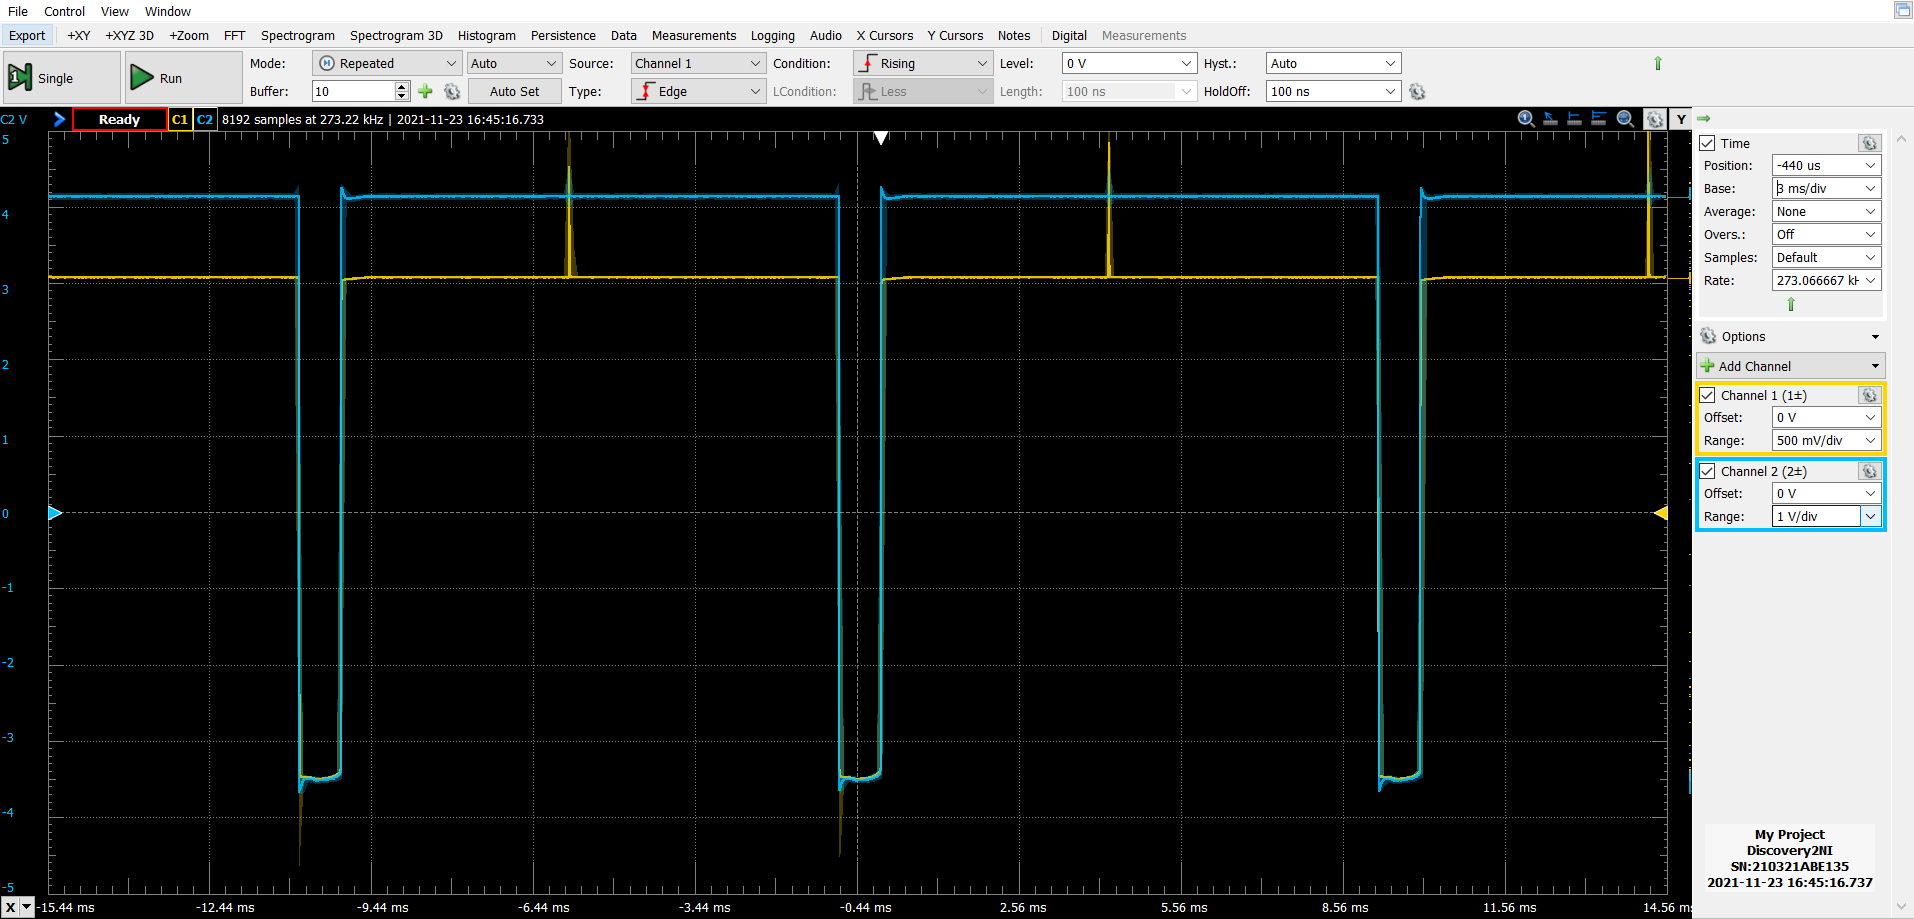
\includegraphics[scale=0.42]{monostabileV+}
	\caption{Acquisizione all'oscilloscopio dell'andamento nel tempo dei
	segnali $v_+ (t)$ (CH1) e $V\ped{out} (t)$ (CH2). \label{fig: mstabilev+}}
\end{figure}

\subsection{Durata dell'impulso generato}
Si è inviata all'ingresso del circuito di trigger un'onda quadra di ampiezza
$V\ped{trig} = 1.99 \pm 0.02 \; \si{\V}$ e frequenza $100 \pm 1.6 \; \si{\Hz}$.

Dunque abbiamo misurato coi cursori le tensioni di saturazione dell'uscita e 
$V_\gamma$ dal livello di tensione costante a cui si trova $v_-$ quando il
circuito è nello stato stabile:
\begin{align*}
V_{OH} &= 4.12 \pm 0.04 \; \si{\V} \quad &V_{OH} &= 4.14 \pm 0.04 \; \si{\V} \\
V_{OL} &= -3.56 \pm 0.03 \; \si{\V} \quad &V_{OL} &= -3.49 \pm 0.03 \; \si{\V} \\
V_{\gamma} &= 547 \pm 6 \; \si{m\V} \quad &V_{\gamma} &= 549 \pm 6 \; \si{m\V}
\end{align*}

E sempre con i cursori si sono misurati i tempi per cui il segnale $V\ped{out}$
rimane ``basso'' in ciascun circuito:
\begin{align*}
t_L &= 767 \pm 10 \;\si{\micro\s} \\
t_L &= 784 \pm 10 \;\si{\micro\s}
\implies \mathrm{dc} = 1 - \frac{t_L}{T} = 92.2 \pm 1.5 \% 
\end{align*}

Il valore atteso per la durata dell'impulso nello stato instabile è legato
al tempo caratteristico in cui si scarica il condensatore $C_1$ dalla
\begin{equation}\label{eq: mstable_Delta}
t\ped{L, exp} = \tau \ln{\left(\frac{1 - V_\gamma/V_{OL}}{1 - q}\right)} =
0.80 \pm 0.03 \; \si{\micro\s}
\end{equation}
Questo risulta compatibile entro l'incertezza con la durata dell'impulso
misurata in uscita dal multivibratore.

\subsection{Analisi del funzionamento del circuito}
Se il condensatore $C_1$ è inizialmente scarico e $V\ped{out} = V_{OH}$, allora
il condensatore in parallelo a $D_1$ si carica fino a quando la d.d.p. tra le
sue armature $V_C \approx V_{\gamma}$. Quindi, poiché $v_- \approx V_{\gamma}$
e $v_+ = \frac{R_{2}}{R_{1} + R_{2}} V\ped{out} \approx \SI{2}{V}$, l'uscita
rimane a livello ``alto''.

Se il condensatore è inizialmente carico (con tensione massima
$v_- \leq V_\gamma$) e se $V\ped{out} = V_{OL}$, allora si scarica fintanto
che vale $v_- \geq v_+ \approx - 1.7 {\V}$. Una volta scarico alla fine
dell'impulso, poiché l'OpAmp è in regime non-lineare, l'uscita commuta
rapidamente (entro i limiti imposti dallo slew-rate) a $V\ped{out} = V_{OH}$;
il condensatore torna a caricarsi e il circuito ritorna alla configurazione
stabile ($v_- \approx V_\gamma$) concludendo il ciclo.

Il sotto-circuito di trigger, formato dal passa-alto $R_4 + C_2$ con il diodo
$D_2$ in cascata, invia all'ingresso non-invertente dell'OpAmp dei picchi di
differenza di potenziale. Questi sono generati grazie al condensatore $C_2$, 
che elimina la componente continua dell'onda quadra $V\ped{trig} (t)$, di cui
ci interessano solamente i fronti ripidi in discesa (e meno in salita).
Infatti è la discesa di $V\ped{trig}$ a generare l'impulso negativo in uscita
dal multivibratore, mentre il fronte di salita è responsabile per i picchi di
tensione positiva che osserviamo in \cref{fig: mstabilev+vtrig}
\begin{figure}[htbp]
	\centering
	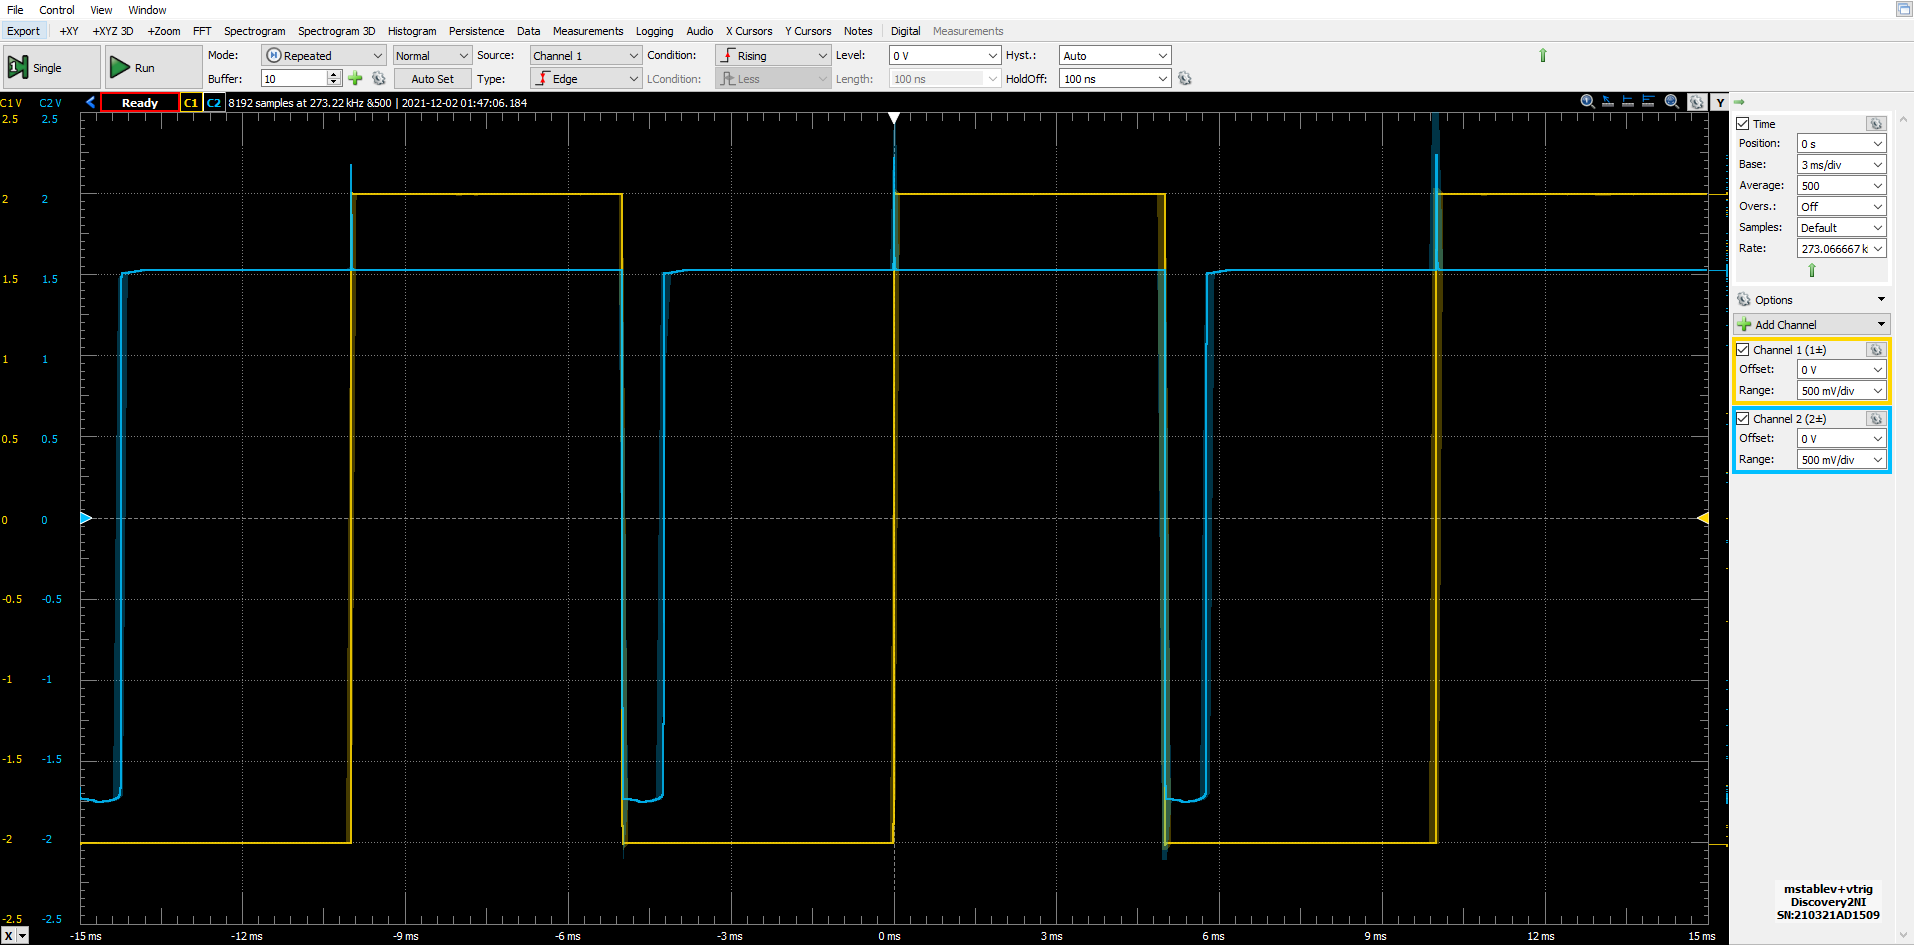
\includegraphics[scale=0.335]{mstablev+vtrig}
	\caption{Acquisizione all'oscilloscopio dell'andamento nel tempo dei
	segnali $V\ped{trig} (t)$ (CH1) e $v_+ (t)$ (CH2).
	\label{fig: mstabilev+vtrig}}
\end{figure}

La risalita del treno d'impulsi in $V\ped{out} (t)$ deve avvenire mentre
$V\ped{trig} (t)$ è ancora costante nel semi-periodo negativo, prima che torni
``alto''. Poiché questa risalita si verifica nel momento in cui $v_- (t)$
assume il suo valore minimo $v_- \approx \frac{1}{2} V_{OL}$ che fa
``scattare'' il comparatore, $C_1$ deve avere il tempo necessario di caricarsi
prima che possa partire una nuova scarica, dunque un nuovo impulso negativo.

Si è quindi tenuta fissa l'ampiezza di $V\ped{trig}$ e se ne è variata la
frequenza. Si osserva che la durata dell'impulso in $V\ped{out}$ rimane
(entro le incertezze di misura) indipendente dalla frequenza del segnale di
trigger, fino a quando la durata dell'impulso è minore del semi-periodo di
$V\ped{trig}$. Al di sopra di questa frequenza critica (sperimentalmente
abbiamo trovato $f\ped{crit} \approx \SI{1}{k\hertz}$) il circuito smette di
funzionare correttamente per durate dell'impulso superiori a
$\frac{1}{2} T\ped{trig} \approx 0.5 \; \si{m\s}$ per via dei tempi di carica
del condensatore $C_1$, come si può vedere in \cref{fig: mstabileflim}.
\begin{figure}[htbp]
	\centering
	\includegraphics[scale=0.335]{mstable950hz}
	\caption{Acquisizione all'oscilloscopio dell'andamento nel tempo dei
	segnali $v_- (t)$ (CH1) e $V\ped{out} (t)$ (CH2) alla frequenza limite
	per cui è possibile pilotare il multivibratore monostabile.
	\label{fig: mstabileflim}}
\end{figure}

Si è variato il duty-cycle dell'onda $V\ped{trig} (t)$ tenendo fissate
frequenza ed ampiezza. Non abbiamo riscontrato una apprezzabile dipendenza
della durata dell'impulso in $V\ped{out} (t)$ dal duty cycle per il range
esplorato tra l'$1 \%$ e il $99 \%$, come era ragionevole aspettarsi, visto che
utilizziamo solamente i fronti di transizione dell'onda quadra.

Infine abbiamo mantenuto costanti frequenza e duty-cycle di $V\ped{trig} (t)$
e ne abbiamo variato l'ampiezza. La durata dell'impulso in $V\ped{out} (t)$
risulta (entro le incertezze sperimentali) indipendente dall'ampiezza del
segnale di trigger per valori di $V\ped{trig}$ maggiori di una certa soglia.
Si è misurato con i cursori l'ampiezza minima al di sotto della quale
il multivibratore non riesce a compiere la transizione alto-basso,
che risulta
\begin{align*}
V\ped{trig}\ap{min} = 768 \pm 6 \; \si{m\V}
\end{align*}
In effetti, se $V\ped{trig}$ è minore di questa soglia ci aspettiamo
che $v_+ (t)$, quindi gli impulsi prodotti dal trigger sovrapposti al segnale
in uscita dal partitore, non siano abbastanza grandi da rendere
$v_d = v_+ - v_- < \SI{0}{\V}$ e quindi far commutare il discriminatore; perciò
$V\ped{out}$ rimane fisso alla tensione di saturazione alta, che
corrisponde a quanto si è osservato dall'esperimento.

%=======================
\section*{Conclusioni e commenti finali}
Si è riusciti a costruire e studiare alcuni dei circuiti più semplici e noti
che fanno uso di amplificatori operazionali in regime non lineare, tra cui:
un amplificatore di carica, un trigger di Schmitt e due multivibratori; uno
astabile e uno monostabile.

In particolare siamo riusciti a descrivere e verificare sperimentalmente il
funzionamento dei circuiti e a caratterizzarne tempi e frequenze
caratteristici; dunque anche i limiti fisici in frequenza, ampiezza e
duty-cycle sia per i segnali in ingresso che nella risposta all'uscita.

%=======================
\section*{Dichiarazione}
I firmatari di questa relazione dichiarano che il contenuto della relazione \`e
originale, con misure effettuate dai membri del gruppo, e che tutti i firmatari
hanno contribuito alla elaborazione della relazione stessa.

\newpage
\appendix
\subsection*{Appendice}\label{sec: appendix}
Consideriamo il circuito formato dal condensatore $C_T$ e dal sotto-circuito
di formazione. La trasformata di Laplace della funzione di trasferimento che
lega $V_s$ a $V\ped{sh}$ per un amplificatore invertente con impedenze
complesse è:
\[
\tilde{A}(s) =
- \frac{\left(\frac{1}{R_1} + s C_F\right)^{-1}}{\frac{1}{s C_T}} =
- \frac{C_T}{C_F} \frac{s}{s + \frac{1}{\tau}}
\]
con $\tau \coloneqq R_1 C_F$. In ingresso inviamo un'onda quadra di periodo
$\mathcal{T} = 2T$ (per il principio di causalità la consideriamo nulla per
tempi $t < 0$) che possiamo scrivere come
\[
V\ped{in}(t) = \sum_{k=0}^{+\infty} (-1)^kf(t - kT)
\]
dove abbiamo definito $f(t) \coloneqq V_s \left[\theta(t) -
\theta(t - T)\right]$, la cui trasformata di Laplace è del tipo
\[
\tilde{f}(s) = V_s\left[\frac{1}{s} - \frac{e^{-sT}}{s}\right]
\]
Per cui possiamo riscrivere la trasformata dell'onda quadra in ingresso
\[
\tilde{V}\ped{in}(s) = \sum_{k=0}^{+\infty} (-1)^k \tilde{f}(s) e^{-kTs} = 
\tilde{f}(s) \sum_{k=0}^{+\infty} (-1)^k e^{-kTs}
\]
ed arrivare alla risposta del circuito in trasformata di Laplace dal
prodotto di convoluzione
\[
\tilde{V}\ped{sh}(s) = \tilde{A}(s) \tilde{V}\ped{in}(s) =  
\tilde{A}(s)\tilde{f}(s) \sum_{k=0}^{+\infty} (-1)^ke^{-kTs} =
\tilde{g}(s) \sum_{k=0}^{+\infty} (-1)^ke^{-kTs} =
\mathcal{L}\left[\sum_{k=0}^{+\infty} (-1)^kg(t - kT)\right](s)
\]
In cui abbiamo introdotto la trasformata della funzione di Green del sistema
\[
\tilde{g}(s) = - V_s \frac{C_T}{C_F} \left[\frac{1}{s + \frac{1}{\tau}} -
\frac{e^{-sT}}{s + \frac{1}{\tau}}\right]
\]
la cui anti-trasformata ha espressione
\[
g(t) = - V_s \frac{C_T}{C_F} \left[e^{-t/\tau}\theta(t) - 
e^{-(t-T)/\tau} \theta(t - T) \right]
\]

Da cui deduciamo la risposta del circuito nel dominio del tempo:
\begin{align}
V\ped{sh}(t) &= - V_s \frac{C_T}{C_F} \left\{ 
\sum_{k=0}^{+\infty} (-1)^k e^{-\frac{t - kT}{\tau}}\theta(t - kT) - 
\sum_{k=0}^{+\infty} (-1)^k e^{-\frac{t - (k+1) T}{\tau}} \theta(t - (k+1)T)
\right\} \\
&= - V_s \frac{C_T}{C_F} \left\{ e^{-\frac{t}{\tau}} \theta(t) -
2 \sum_{k=1}^{+\infty} (-1)^k e^{-\frac{t - kT}{\tau}}
\theta(t -  kT) \right\}
\label{eq: antlaplace}
\end{align}
Finalmente, trascurando il transiente iniziale $(k = 0)$ e supponendo
che\footnote{Qui stiamo assumendo che la somma sia ben definita, come si può
verificare dal fatto che vale (a meno di costanti fisiche)
\[
\sum_{k \geq 0} \theta(t-k) e^{-(t-k)} =
\sum_{k=0}^{\lfloor t \rfloor} e^{-(t-k)} \leq \frac{e}{e-1} e^{-\{t\}}.
\]}
$\tau \ll T$, possiamo sviluppare l'\cref{eq: antlaplace} per avere la forma 
d'onda attesa in uscita dallo shaper
\begin{align}\label{eq: Vshaper}
V\ped{sh}(t) &\approx 2 V_s \frac{C_T}{C_F} \sum_{k=1}^{+\infty} 
(-1)^{k} e^{-\frac{t - kT}{\tau}} \theta(t - kT) \nonumber\\
&\approx  2 V_s \frac{C_T}{C_F} \sum_{k=1}^{+\infty} 
(-1)^{k} e^{-\frac{t - kT}{\tau}} \chi_{[kT, (k+1)T]}(t)
\end{align}
\end{document}
